\chapter{Analyzing cross-species genetic networks to predict disease-associated genes: application on Plasmodium falciparum malaria}\label{chap:malaria}
\section{Motivating Example}\label{motivating}


Malaria is the most deadly parasitic
infectious disease

Figure \ref{code} shows a short function {\it harmean}, which correctly calculates the harmonic mean of two floating point numbers, in the middle column and shows a faulty version of {\it harmean} in the rightmost column.  (In real fault localization scenarios only the faulty code is usually available.)  We injected a fault into statement $s_3$ by adding a floating point number $c$ to the original expression $a*b$.  Given a pair of inputs $(a,b)$, the faulty version of $s_3$ produces an erroneous value for the variable $x$.  This value may propagate to statement $s_8$ and, via the variable $r$, cause an incorrect return value at statement $s_9$.  We use $r_{correct}$ and $r_{faulty}$ to denote the return value of the correct code and faulty code, respectively.  Let us assume that the faulty version of {\it harmean}, like many numerical programs, is considered to fail if the output error exceeds a predefined threshold $\epsilon$, that is, if

\begin{equation*}\label{threshold}
outerr = |{r_{correct}} - {r_{faulty}}| > \varepsilon
\end{equation*}

\begin{figure*}[!thpb]
\centering
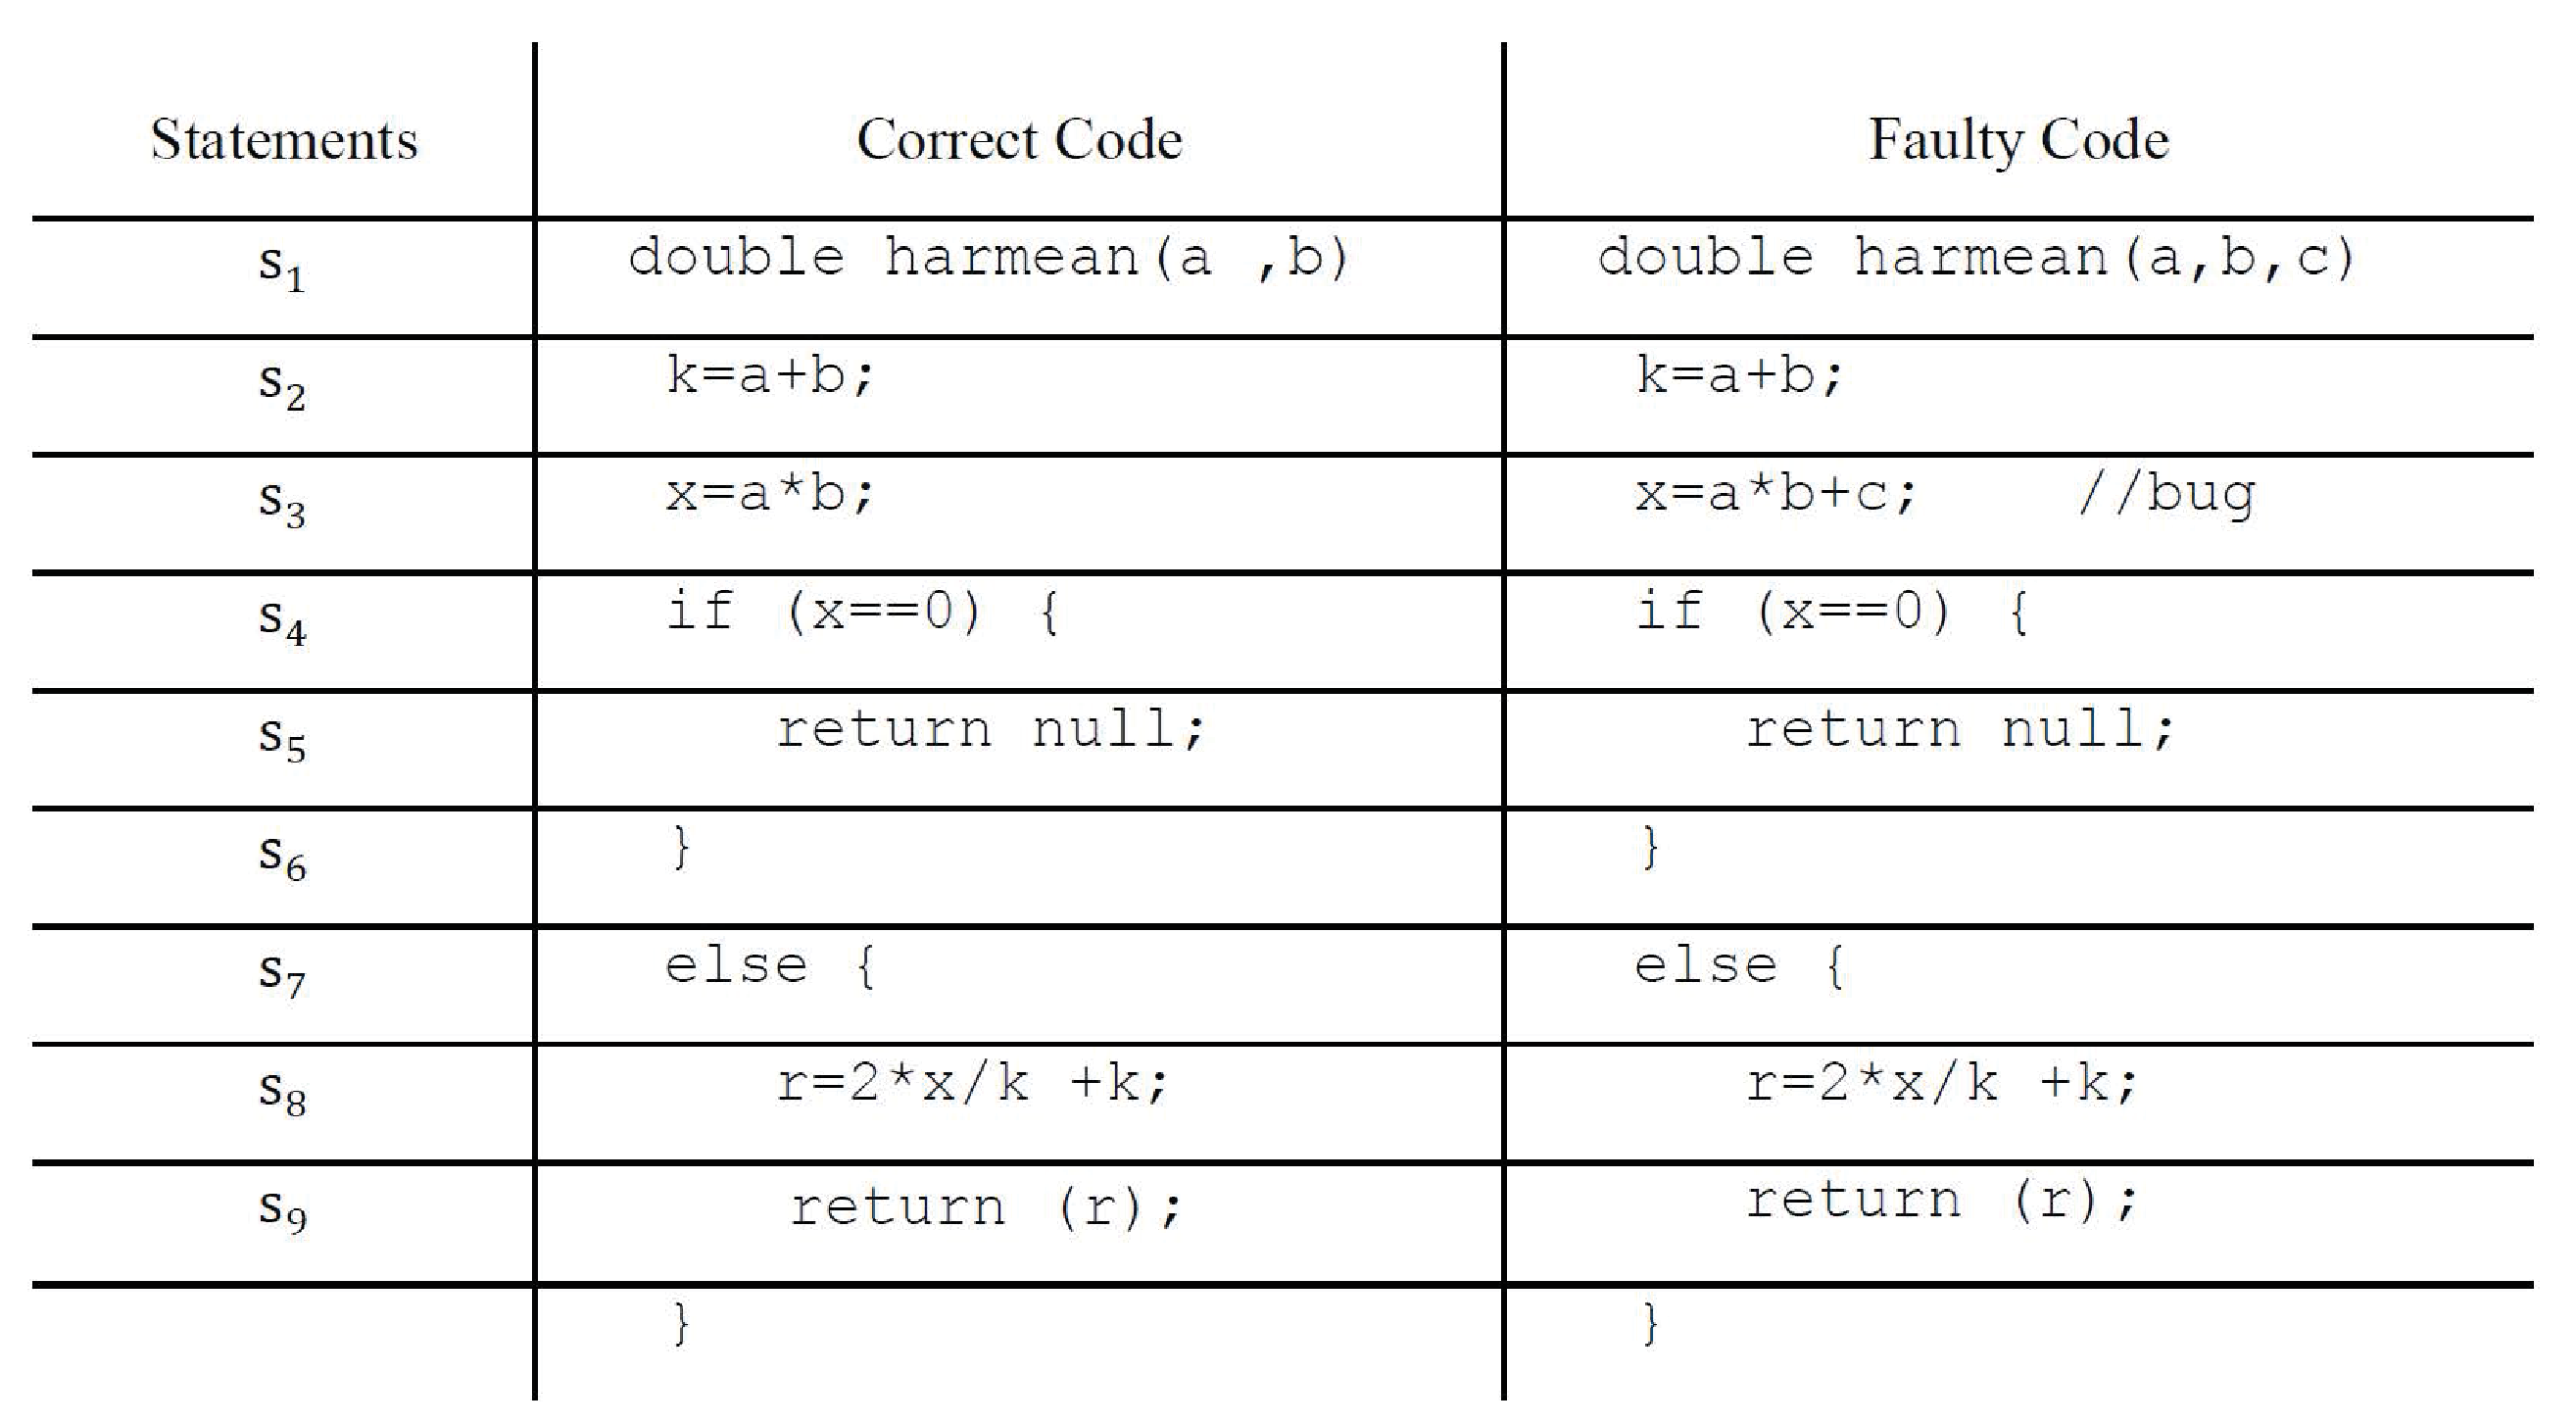
\includegraphics[width=0.8\textwidth]{MotivatingExample.eps}
\caption{Motivating Example}
\label{code}
\end{figure*}

Our goal is to automatically localize faults in numerical expressions, given variable-value profiles and expected outputs.  In the faulty code of Figure \ref{code}, there are three numerical expressions, in statements $s_2$, $s_3$ and $s_8$ , which define variables $k$, $ x$, and $r$.  A simple approach to detecting which expressions contain numerical faults is to obtain a ``suspiciousness" score for each numerical expression by calculating a measure of the statistical association between the values of the expression and the output error. This na\"{i}ve approach has two potential problems, however.  First, erroneous values due to a fault in one expression may propagate to other, correct expressions, causing them to receive high suspiciousness scores.  For example, in Figure \ref{code} the fault in statement $s_3$ causes variable $x$ to have erroneous values that propagate to statement $s_8$ and cause variable $r$ to have erroneous values. Consequently, the output error of {\it harmean} is associated with the values computed by both $s_3$ and $s_8$, even though $s_8$  is correct.  This problem, which is an instance of {\it confounding bias} (or {\it confounding}), is due to the fact that the computation of $x$ at $s_3$ is a {\it common cause} of program failure and of the computation of $r$ at $s_8$.  A na\"{i}ve measure of the association of $r$ with the output error, which does not account for confounding, will reflect both the true causal effect of $r$ on failure and the biasing effect of the confounder $x$ on $r$ and $outerr$.

The second problem with the na\"{i}ve approach is that common association measures like Pearson's correlation coefficient \cite{Philip2012} are often inadequate to measure the causal effect of a numerical expression on a program's output error, even without confounding.  For the example in Figure \ref{code},  $outerr=|r_{correct}-r_{faulty} |=|2c/(a+b)|$.  If $a=1$ and $b=0$, then $outerr=2|c|$ and $x=c$.  By definition, the correlation between $x$ and $outerr$ is:
\begin{equation*}\label{correlation}
%corr(x,outerr) = \frac{{{\mathop{\rm cov}} (x,outerr)}}{{{\sigma _x}{\sigma _{outerr}}}} = \frac{{{\mathop{\rm cov}} (c,2|c|)}}{{{\sigma _x}{\sigma _{outerr}}}}
corr(x,outerr) = \frac{{{\mathop{ cov}} (x,outerr)}}{{{\sigma _x}{\sigma _{outerr}}}} = \frac{{{\mathop{ cov}} (c,2|c|)}}{{{\sigma _x}{\sigma _{outerr}}}}
\end{equation*}
where $cov(x,outerr)$ is the covariance between $x$ and $outerr$ and where $\sigma_x$ and $\sigma_{outerr}$ are the standard deviations of $x$ and $outerr$, respectively.  Using basic covariance identities, we find that $cov(c,2|c|)=2cov(c,|c|)=2E[(c-\mu_c )(|c|-\mu_{|c|})]$, where $\mu_c$ and $\mu_{|c|}$ are the means of $c$ and $|c|$ respectively.  If the distribution of variable $c$ is symmetric about 0, $cov(c,|c|)$ is equal to 0, and so is $corr(x,outerr)$. Therefore, $corr(x,outerr)$ can be 0, even though the statement defining $x$ contains a fault.

NUMFL is intended to address the aforementioned problems and to provide less-biased estimates of the {\it failure-causing effect} of a numerical expression.  We now map the causal variables defined in the Introduction to the variables in our example:
\begin{enumerate}
\item 	Treatment variable $T_e$ is the variable defined in a numerical expression $e$.  In Figure \ref{code}, variables $k$, $x$ and $r$ are the treatment variables associated with statements $s_2$, $s_3$ and $s_8$, respectively.
	\item Outcome variable $Y$ is the absolute difference between the output of the faulty program and the expected (correct) output.  For the example, $Y$ is $outerr$.
\item $X$ represents the confounding variables, which are each causes of both treatment $T_e$ and outcome $Y$. For example, in the numerical expression $r=2*x/k$, the variables $x$ and $k$ are confounders because they each influence the values of both the treatment $T_e=r$ and the outcome $Y=outerr$.

\end{enumerate}

Figure \ref{dag1} shows the causal relationships between treatment, outcome, and confounding variables.
\begin{figure*}[!thpb]
\centering
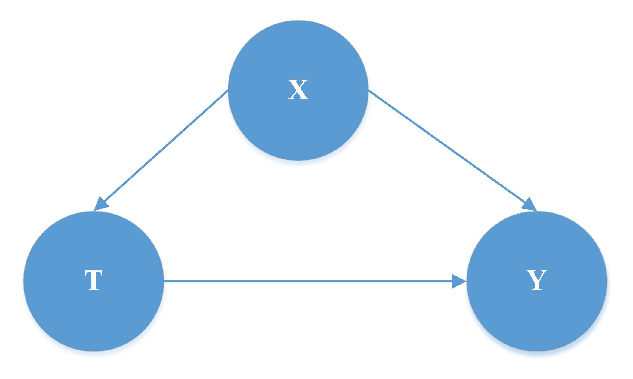
\includegraphics[width=0.5\textwidth]{CausalDAG1.eps}
\caption{Causal diagram of treatment, outcome, and confounder.}
%\vspace{-.5cm}
\label{dag1}
\end{figure*}


\section{BACKGROUND}\label{background}
\subsection{Causal Inference Methodology}\label{IIIA}
Causal inference methodology \cite{Pearl2003} has emerged in recent decades from research in a number of applied fields, to provide a basis for making valid inferences, from experimental or observational data, about the causal effects of specified treatments or exposures upon outcomes of interest.  Data about study variables is augmented with background knowledge about the causal relationships among variables, which is represented as {\it causal DAG}: a directed acyclic graph, in which nodes correspond to variables and in which there is an edge $A \to B$ if $A$ is an actual or assumed cause of $B$.  Causal inference theory establishes graph-theoretic conditions, such as Pearl's Backdoor Criterion \cite{Pearl2003}, under which a given causal effect can be estimated statistically without confounding or other forms of bias such as selection bias and measurement bias.



\subsection{Ordinary Propensity Scores}\label{IIIB}
Consider a treatment variable $T$ with two possible values 1 and 0.  (These values may indicate ``treated" and ``untreated", respectively, or they may indicate alternative treatments.)  One of the reasons that ideal randomized experiments, when they are feasible, are often considered the ``gold standard" for the design of causal inference studies \cite{Grossman2005} is that randomization makes it likely that the joint distribution of the covariates of the units with $T=1$ is similar to the covariate distribution of the units with $T=0$.  Such similarity, which is called {\it covariate balance} \cite{Rosenbaum1983}, implies that the two groups of units are comparable with respect to the values of confounding covariates, so that any difference in average outcomes of the groups is likely to be due to the treatment variable and not to confounding.  In randomized experiments, covariate balance is a consequence of the fact that the randomized treatment variable is {\it independent} of the covariates.

\begin{figure*}[!thpb]
\centering
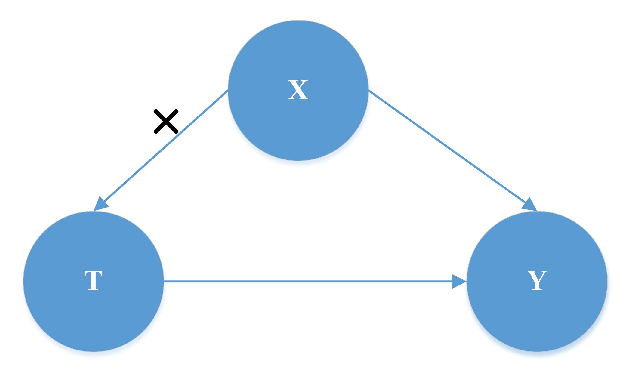
\includegraphics[width=0.5\textwidth]{CausalDAG2.eps}
\caption{Matching units based on their propensity scores breaks the link between cofounding variables and treatment.}
%\vspace{-.5cm}
\label{dag2}
\end{figure*}

An important approach to achieving covariate balance in observational studies is the use of (ordinary) {\it propensity scores} \cite{Rosenbaum1983}.  For a binary treatment variable $T$ and a vector of covariates $\pmb{X}$, the propensity score $Pr(T=1|\pmb{X}=\pmb{x})$ is the conditional probability of treatment $T=1$ given that the observed value of $\pmb{X}$ is $\pmb{x}$.  It has been shown that the propensity score is a {\it balancing score} in the sense that comparison groups with similar propensity scores tend to have similar covariate distributions \cite{Rosenbaum1983}.  True propensity scores are generally unknown, but they can be estimated from data about study units' actual treatment and covariate values.

Suppose that for each unit $i$ examined in an observational study, we have recorded the values of a binary treatment variable ${T_i} \in \{ 0,1\} $ and a vector of covariates ${\pmb{X}_i}$ .  We can use a parametric model ${\pi _{\pmb\beta} }({\pmb{X}_i})$ to estimate the propensity score for unit $i$.  One choice is the logistic model:

\begin{equation*}
{\pi _{\pmb\beta} }({X_i}) = Pr({T_i} = 1|{\pmb{X}_i}) = \frac{{\exp ({\pmb{X}_i}^\prime \pmb\beta )}}{{1 + \exp ({\pmb{X}_i}^\prime \pmb\beta )}}
\end{equation*}

We can estimate the parameter $\pmb\beta$ using maximum likelihood estimation \cite{Silvapulle1981}, which involves maximizing the log-likelihood function:

\begin{equation}\label{eq1}
{\pmb{\hat \beta} _{MLE}} = \arg \;\max \sum\limits_{i = 1}^N {{T_i}\log \left\{ {{\pi _{\pmb\beta} }({\pmb{X}_i})} \right\} + (1 - {T_i})} \log \left\{ {1 - {\pi _{\pmb\beta} }({\pmb{X}_i})} \right\}
\end{equation}

With the fitted model, we can estimate the ordinary propensity score  ${\pi _{\pmb\beta}}({\pmb{X}_i})$ for each observed unit.

After the propensity score model is estimated, covariate balance may be achieved by matching units based on their estimated propensity scores \cite{Rosenbaum1983}.  For example, each unit with $T=1$ can be matched to a unit with $T=0$ that has a similar estimated propensity score, if such a unit exists.  As illustrated in Figure \ref{dag2}, matching units based on their propensity scores breaks the link between the confounding variables and the treatment variable.

Ordinary propensity scores are not applicable to continuous treatment variables, however.  To address confounding of SFL scores for numerical expressions, we consider two variants of ordinary propensity scores that can accommodate continuous (and integer) treatment variables.  The first variant is the Generalized Propensity Score (GPS) proposed by Imai and Van Dyk \cite{Imai2004}.  The second variant is the Covariate Balancing Propensity Score (CBPS) proposed by Imai and Ratkovic \cite{Imai2014}.  Since CBPS is quite new, it has not been established whether it is superior to GPS.  Hence, we shall present and evaluate two versions of NUMFL, denoted NUMFL-GPS and NUMFL-CBPS, which are based on GPS and CBPS, respectively.  First, though, we briefly describe GPS and CBPS in the next two subsections.

\subsection{Generalized Propensity Score (GPS)}\label{IIIC}
The {\it Generalized Propensity Score} proposed by Imai and van Dyk \cite{Imai2004} is intended for use with any kind of treatment variable, including continuous ones.  Let ${p_{\pmb{\psi}} }(T|\pmb{X})$  be a model, with parameters $\pmb{\psi}$, of the {\it conditional probability density function} (p.d.f.) of the treatment variable $T$ given the covariate vector $\pmb{X}$.  The GPS for a specific unit with treatment level $T=t$ and covariate values $\pmb{X=x}$ is the density value $r = {p_{\pmb\psi} }(T = t|{\pmb X} = {\pmb x})$.  Imai and van Dyk \cite{Imai2004} require that the model ${p_{\pmb{\psi}} }(T|\pmb{X})$ has a {\it unique parameter} ${\pmb\theta}  = \pmb{\theta _\psi }(X)$ such that ${p_{\pmb{\psi}} }(T|\pmb{X})$ {\it depends on} $\pmb X$ {\it only through} $\pmb \theta$.  For example, if the treatment is represented by a {\it linear Gaussian model} $T|\pmb{X} \sim {\cal N}(\pmb{X}'{\pmb \beta} ,{\sigma ^2})$ with mean $\pmb{X}'{\pmb \beta}$  (the scalar product $\pmb{X}$-transpose times $\pmb{\beta}$) and variance $\sigma ^2$, so that $\pmb{\psi}  = \left( {\pmb{\beta} ,{\sigma ^2}} \right)$, then $\pmb{\theta}  = \pmb{X}'\pmb{\beta} $ (here $\pmb{\theta} $ is scalar).  The model parameters $\pmb{\psi}$, $r$, $\pmb{\theta}$, $\pmb{\beta}$, etc. are estimated from data; the corresponding estimates are denoted with by $\hat {\pmb\psi} $, $\hat r$, $\hat{ \pmb{\theta}} $, $\hat{ \pmb{\beta}}$, etc..  In Imai and van Dyk's approach, it is the values of the parameter estimate ${{\hat{\pmb{\theta}} }_{\hat{ \pmb{\psi}} }}(\pmb{X})$ that are used to control confounding, rather than the values of ${p_{\hat{ \pmb{\psi}} }}(T|\pmb{X})$ themselves.

\subsection{Covariate Balancing Propensity Score (CBPS)}\label{IIID}
Section \ref{IIIB} explained that the ordinary propensity score is a balancing score and that it can be estimated from data using a parametric statistical model.  However, if the propensity score model ${\pi _{\pmb \beta} }({\pmb{X}_i})$  is {\it misspecified}, matching on the estimated propensity scores (and related techniques) may fail to balance the covariates, yielding biased estimates of causal effects. To address this problem, Imai and Ratkovic proposed the {\it Covariate Balancing Propensity Score} (CBPS), which is robust to mild misspecification of the propensity score model \cite{Imai2014}.
The CBPS optimizes covariate balance by modifying the estimation procedure for parameter $\pmb{\beta}$ .  Differentiating equation \eqref{eq1}, equating the result to zero, and taking expectations, we have \cite{Imai2014}
\begin{equation}\label{eq2}
E\left\{ {\frac{{{T_i}{{\pi '}_{\pmb \beta} }({\pmb{X}_i})}}{{{\pi _{\pmb \beta} }({\pmb{X}_i})}} - \frac{{(1 - {T_i}){{\pi '}_{\pmb \beta} }({\pmb{X}_i})}}{{1 - {\pi _{\pmb \beta} }({\pmb{X}_i})}}} \right\} = 0,
\end{equation}
where ${\pi '_{\pmb \beta} }({\pmb{X}_i}) = \partial {\pi _{\pmb \beta} }({\pmb{X}_i})/\partial \pmb{\beta}$.  Equation \eqref{eq2} is called a {\it balancing condition} or a {\it moment condition} \cite{Imai2014}.  (The mean of a random variable is its ``first moment" \cite{Rosenblueth1981}.)  In CBPS, the balancing condition is generalized as
\begin{equation}\label{eq3}
E\left\{ {\frac{{{T_i}{{\tilde {\pmb X}}_i}}}{{{\pi _{\pmb \beta} }({\pmb{X}_i})}} - \frac{{(1 - {T_i}){{\tilde {\pmb X}}_i}}}{{1 - {\pi _{\pmb \beta} }({\pmb{X}_i})}}} \right\} = 0,
\end{equation}
where ${\tilde {\pmb X}_i} = f({\pmb{X}_i})$ represents a vector-valued function of the covariates $\pmb{X}_i$. To ensure that the first moment of each covariate is balanced, even when the model is misspecified, we can set ${\tilde {\pmb X}_i} = {\pmb{X}_i}$. CBPS employs a parameter estimation framework called the {\it generalized method of moments} (GMM) \cite{Hansen1982}, which is based on solving moment-condition equations for the parameters of interest and substituting sample moments for unknown population moments. Imai {\it et al}. extended CBPS to treatments with $K>2$ integer values, using a $multinomial\;model$ for the conditional probability of treatment given the covariates. We adapted this approach slightly to make it applicable to value-based fault localization (see Section \ref{IVB}), and we evaluate CBPS in NUMFL as an alternative to GPS .

\section{TWO VERSIONS OF NUMFL}\label{twoversion}
In this section, we define two versions of NUMFL, NUMFL-GPS and NUMFL-CBPS, and explain how they are used to reduce confounding bias during estimation of a numerical expression's {\it average failure-causing effect} (AFCE). Intuitively, an aggregate measure of the failure-causing effect of a numerical expression $e$ should summarize the effects on output errors of evaluating $e$ over a sample of program runs that each cover or reach $e$. Accordingly, in causal inference the designated ``treatment" variable $T_e$ should reflect the values produced by individual evaluations of $e$. (Of course $e$ may be evaluated repeatedly in a single program run, due to iteration.) Runs that do not reach $e$ are {\it not relevant} to such a measure. This is unlike measures of the failure-causing effect of covering a statement $s$ at least once during a run (e.g., \cite{Jones2002}), which contrast runs that cover $s$ with runs that don't cover $s$. With such measures, the treatment variable indicates whether or not $s$ was covered during a given run.

Recall that confounding of the causal effect of a treatment variable $T$ upon an outcome variable $Y$ is bias that is due to the presence of one or more common causes of $T$ and $Y$. The influence of such a common cause $X$ can make the effect of $T$ on $Y$, as reflected by a na\"{i}ve measure of statistical association, appear to be stronger or weaker than it really is. As mentioned in Section \ref{IIIB}, ordinary propensity scores cannot be used in causal inference to control confounding when the treatment variable is continuous.  Since the ``treatments" that NUMFL deals with are the values of numeric program variables, we instead define and evaluate two versions of NUMFL, namely NUMFL-GPS and NUMFL-CBPS, that are based respectively on GPS and CBPS, the two generalizations of ordinary propensity scores described in Sections \ref{IIIC} and \ref{IIID}.

\subsection{NUMFL-GPS}\label{IVA}
As with ordinary propensity scores, GPS is used to control for statistical associations between the treatment variable and confounding covariates, which in the case of NUMFL are variables used (read) in a numeric expression $e$ whose AFCE we wish to estimate. In general, these program variables are potential confounders because they may contain erroneous values just before expression $e$ is evaluated, due to faults in previously evaluated expressions. If these erroneous values cause program failures (that is, ``coincidental correctness" does not occur) the result of evaluating $e$ may be strongly associated with failures even if $e$ is correct, unless steps are taken to control confounding. In NUMFL, therefore, when estimating the AFCE of $T_e$ on the output error $Y$, we control for the values of the variables used in $e$.  (Those familiar with Pearl's Backdoor Adjustment Criterion \cite{Pearl2003} should note that this breaks any backdoor paths between $T_e$ and $Y$ in the acyclic data flow graph induced by a program execution.)

\subsubsection{Control of Confounding.}
For a given numerical expression $e$ in a program, NUMFL-GPS currently fits a linear
Gaussian GPS model ${{\pmb T}_e}|{{\pmb X}_e} \sim N({\pmb X}_e'{{\pmb \beta} _e}, \sigma _e^2)$ , where the treatment variable $T_e$ represents the result of evaluating $e$ (once) and where the possibly confounding covariates in the vector $\pmb{X}_e$ represent the corresponding values of the program variables used in evaluating $e$. Observe that one program run may generate multiple values of $T_e$ and $\pmb{X}_e$, due to iteration. To reduce profiling overhead, these may be sampled rather than recorded exhaustively. We currently sample only the values from the {\it last iteration} of a loop.

Applying GPS in NUMFL entails the following three steps:
\begin{enumerate}
\item 	Given a sample of observed values for the treatment variable $T_e$ and for the covariates $\pmb{X}_e$, fit a linear regression model $T_e=\pmb{X}_e' \pmb{\beta}_e$ to obtain the estimated parameter vector $\hat {\pmb{\beta}}_e$.
\item For each observed value ${\pmb x}_{e,i}$ of $\pmb{X}_e$, compute the estimate ${{\hat \theta }_{e,i}} = {\pmb{x}_{e,i}}'{{\hat {\pmb{\beta}} }_e}$.
\item Group observations with the same or similar values of $\hat{\theta}_{e,i}$ into $m$ subclasses of roughly equal size.
\end{enumerate}

The regression model fitted in the first step characterizes how the values of the covariates in $\pmb{X}_e$ influence the value of the treatment variable $T_e$.  In the second step, $\hat{\theta}_{e,i}$ estimates this influence for a particular value $\pmb{x}_{e,i}$ of $\pmb{X}_e$.  The scalar $\hat{\theta}_{e,i}$ summarizes the influence of the vector value $\pmb{x}_{e,i}$ on the treatment, and hence $\hat{\theta}_{e,i}$ may be used in place of $\pmb{x}_{e,i}$ for confounding control. Accordingly, in the third step, each subclass of observations with similar $\hat{\theta}_{e,i}$ values corresponds to a set of $\pmb{x}_{e,i}$ values that influence the treatment similarly. Thus, within each subclass, there is little or no association between confounders and the treatment variable $T_e$.

To illustrate this procedure, we refer again to the faulty version of the function {\it harmean} in Figure \ref{code}.  Statement $s_8$ is $r=2*x/k +k$. To control possible confounding of the average failure-causing effect of $r$ by the variables $x$ and $k$, we first fit a linear model $r=\beta_1 z+\beta_2 k$, where $z=x/k$, using a sample of corresponding observed values $(r_i,x_i,k_i)$. Second, we apply the fitted model to each pair $(x_i,k_i)$ to obtain a predicted value $\hat \theta_i$.  Third, we group the observations with similar $\hat \theta_i$ values into subclasses. This can be done by sorting the $\hat \theta_i$ into descending order and partitioning the sorted values into $m$ roughly equal-size bins.

Although GPS can control confounding bias caused by multiple confounding covariates, there is one challenge to applying it in NUMFL-GPS. If the dimension of $\pmb{X}_e$ is high, the first step of GPS requires a large number of observations to fit a suitable regression model.  In practice, a numerical expression defined by a statement could contain more than 10 confounders, but the number of tests may not be large enough to fit the regression parameters with adequate precision. Thus, to apply GPS, we need to control the dimension of confounding variables.

To address this problem, we $decompose$ a complex numerical expression into several subexpressions, each involving operators with the same precedence level.  For example, a numerical statement $a=(b+c+d)*e$ will be decomposed into two subexpressions: (1) $temp=b+c+d$ and (2) $a=temp*e$.  Here, $temp$ is a temporary variable that plays the role of the treatment variable for subexpression (1) and the role of a possible confounder for subexpression (2). Thus, each subexpression has fewer confounding variables and a relatively simple structure.  For each subexpression, we use GPS to control confounding bias and then estimate the subexpression's AFCE.

\subsubsection{Failure-causing Effect Estimation.}
Within each of the subclasses created by grouping observations with similar $\hat \theta_i$ values, the treatment values $T_{e,i}$ should be largely independent of the covariate values $\pmb{X}_{e,i}$, provided that the GPS model is adequate. Hence, the relationship between the treatment variable $T_e$ and the outcome variable $Y$ should be nearly unconfounded in each subclass. If this relationship is roughly linear in each subclass, we can estimate the expected dose-response function $E[Y|T_e]$ {\it within a particular subclass} using a simple linear regression model \cite{Zhao2013}:
\begin{equation}\label{lrm}
Y=\gamma_eT_e+b
\end{equation}
Recall that $Y$ is the absolute difference between the output of the faulty program and the expected (correct) output. In equation \eqref{lrm}, $b$ is a constant intercept. The coefficient $\gamma_e$ is the slope of $E[Y|T_e]$. It indicates how much the expected value of the outcome variable changes when the treatment value increases by one unit. The slope coefficient $\gamma_e$ can be estimated by the least-squares estimator $\hat \gamma_e$:
\begin{equation}\label{ls}
\hat \gamma_e=({\pmb t}_e'{\pmb t}_e)^{-1}{\pmb t}_e'{\pmb y},
\end{equation}
where $\pmb{t}_e'$ is the transpose of the vector of treatment values and where $\pmb y$ is the vector of outcome values (output errors).

Intuitively, an association measure used as an SFL suspiciousness metric for numerical programs should, when applied to a numerical expression $e$, reflect the likelihood that $e$ is faulty.  Although the coefficient estimate $\hat \gamma_e$ summarizes the dose-response function, it is not an adequate SFL metric, because of the {\it symmetry} of many numerical errors. For example, suppose that $Y=|T_e |$.  Since the output error $Y$ is completely determined by $T_e$, expression $e$ should receive a high suspiciousness score. However, if the value of $T_e$ is distributed symmetrically around zero, then $\hat \gamma_e$ will be close to zero, which suggests misleadingly that $e$ has no causal effect on program failures.

To derive a better suspiciousness metric, we first analyze the relationship between a numeric fault and the DRF slope estimator $\hat \gamma_e$. Assume that the numeric expression $e$ has a fault, which results in erroneous treatment values represented by the treatment variable $T_e^f=T_e$.  Let the treatment variable $T_e^c$ represent the corresponding treatment values in the correct program. Then we have $T_e^f=T_e^c+\varepsilon_e$, where $\varepsilon_e$ is a treatment error term.  Then $\hat \gamma_e $ may be decomposed as follows:

\begin{equation}\label{decomp}
\begin{array}{l}
{{\hat \gamma}_e} = {({{\pmb t}_e^f}'{\pmb t}_e^f)^{ - 1}}({\pmb t}_e^c + {{\pmb \varepsilon} _e})'{\pmb y}\\
 = {({{\pmb t}_e^f}'{\pmb t}_e^f)^{ - 1}}{{\pmb t}_e^c}'{\pmb y} + {({{\pmb t}_e^f}'{\pmb t}_e^f)^{ - 1}}{{\pmb \varepsilon} _e}^\prime {\pmb y}\\
 = {{\hat \gamma}_e}^c + {{\hat \gamma}_e}^f,
\end{array}
\end{equation}
where $\pmb{t}_e^f$, $\pmb{t}_e^c$, and ${\pmb \varepsilon}_e$ are the vectors of sample values for $T_e^f$, $T_e^c$, and $\varepsilon_e$, respectively, and where ${{\hat \gamma}_e}^c  = {({{\pmb t}_e^f}'{\pmb t}_e^f)^{ - 1}}{{\pmb t}_e^c}'{\pmb y} $ and ${{\hat \gamma}_e}^f = {({{\pmb t}_e^f}'{\pmb t}_e^f)^{ - 1}}{{\pmb \varepsilon} _e}^\prime {\pmb y}$. The component $\hat \gamma _e^f$ of ${\hat \gamma _e}$ characterizes the causal relationship between the treatment error $\varepsilon_e$ and the output error $Y$. If $\varepsilon_e$ is symmetrically distributed then the contributions to $\hat \gamma _e^f$ of the positive and negative values of $\varepsilon_e$ will tend to cancel each other, since $Y$ is an absolute value, leaving $\hat \gamma _e^f$ close to zero.

We have considered two possible approaches to this problem.  We call the first of these a {\it dual linear regression model} (DLRM).  The basic idea of DLRM is simple: compute
$|\hat \gamma _e^f|$ separately for positive $\varepsilon_e$ and for negative $\varepsilon_e$ and then add the two resulting values.  (Using the absolute values of the two estimates ensures that they do not cancel each other.)  However, although the values of $T_e$ are known, the values of $ T_e^c$ and $\varepsilon_e$ are unknown, so $|\hat \gamma _e^c|$ and $|\hat \gamma _e^f|$ cannot be estimated individually.  This issue can be addressed given the following assumptions:\\
\newline
\textit{ \textbf{ Assumption 1}: If expression $e$ is faulty then within each GPS subclass the variance of $ T_e^c$ is much smaller than the variance of $\varepsilon_e$.}\\
\textit{ \textbf{ Assumption 2}: If expression $e$ is faulty then within each GPS subclass, $\varepsilon_e$ is symmetrically distributed about zero.}\\
\newline
Assumption 1 implies that the error  $\varepsilon_e$ is responsible for most of the variance of treatment variable $T_e$ within a subclass.  We have observed that this is often the case. Assumption 2 asserts that the previously mentioned issue with symmetrically distributed treatment errors pertains generally.

Given these two assumptions, using DLRM involves the following steps, which are applied separately to each GPS subclass:
\begin{enumerate}
\item Sort the values of the treatment variable $T_e$ into descending order.  Then split the data into two subsets which contain the values that are larger and smaller than the median value, respectively.
\item 	Estimate the slope of $E[Y|T_e]$ in each subset separately using linear regression model (1).
\item 	Summarize the failure-causing effect of $T_e$ by adding the two estimated slopes’ absolute values.
\end{enumerate}
Under Assumption 1, if expression $e$ is faulty then $T_e^c$ can be viewed as a constant relative to $\varepsilon_e$ within a subclass, so that a large value of $T_e$ corresponds to a large $\varepsilon_e$.  This implies that  $T_e$   and $\varepsilon_e$ have the same sorted order. Assumption 2 implies that splitting the treatment data at its median value separates the treatments with positive $\varepsilon_e$ values from the treatments with negative $\varepsilon_e$ values.  Step 3 prevents the two causal effect estimates from cancelling each other out. Figure \ref{DRF_curves} (a) shows the DRF curve of the DLRM.

In practice, the distribution of $\varepsilon_e$  is usually unknown, so it is quite uncertain whether Assumption 2 holds.  To address this issue, we have used an alternative to DLRM based on a {\it quadratic regression model} [18], which we shall refer to as QRM.   QRM is more flexible than DLRM, because it does not require sorting and splitting the data within subclasses.  It is based on the following alternative to Assumption 2:\\
\newline
\textit{ \textbf{ Assumption 3}: Executions with large absolute treatment errors $\left| {{\varepsilon _e}} \right|$ have larger output errors Y than executions with small values of $\left| {{\varepsilon _e}} \right|$.}\\
\newline
We have observed that this assumption often holds.  If both Assumption 1 and Assumption 3 hold, the failure-causing effect of $T_e$ on $Y$ can be estimated by fitting a quadratic regression model $Y = \varsigma T_e^2 + \eta {T_e} + c$  . Figure \ref{DRF_curves} (b) shows the dose-response curve of QRM, which clearly reflects Assumption 3.  We use the fitted value $\hat \zeta $ of the coefficient $ \zeta $ as the AFCE estimate within each subclass.
\vspace{-0.1cm}

\begin{figure*}[!thpb]
\centering
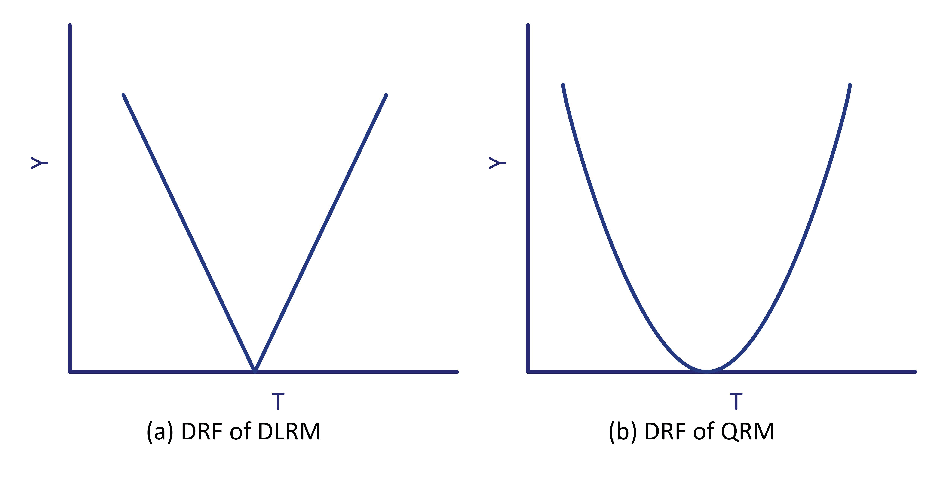
\includegraphics[width=0.7\textwidth]{DRF_curves.eps}
\caption{Matching units based on their propensity scores breaks the link between cofounding variables and treatment.}
%\vspace{-.5cm}
\label{DRF_curves}
\end{figure*}
\vspace{-0.1cm}

Finally, we chose to use the absolute value of fitted a regression coefficient's $t$-statistic [19] as a suspiciousness score, rather than the coefficient itself, because we wish to ``penalize" coefficients with large standard errors.  We use $\left| t \right|$ to denote the absolute value of the $t$-statistic for a fitted coefficient $\hat \beta $: $\left| t \right| = |\hat \beta /std ( {\hat \beta })|$ , where $std(\hat \beta)$ is the standard error of $\hat \beta$.  Thus, for DLRM the failure-causing effect of treatment $T_e$ is estimated by the summation of two linear regression models'$\left| t \right|$ values for the fitted slope coefficient ${{\hat \gamma }_e}$.  For QRM, this effect is estimated by the $\left| t \right|$ value of the estimated coefficient ${\hat \zeta }$ of the quadratic term of the regression model.

\renewcommand{\algorithmicrequire}{\textbf{Input:}}
\renewcommand{\algorithmicensure}{\textbf{Output:}}
\begin{algorithm}
  \captionof{figure}{ {\it NUMFL} Algorithm}\label{NUMFLalg}

  \begin{algorithmic}[1]
    \Require Subexpression value table $E=[T_e, \pmb{X}_e]$, with all values standardized, and type of model $M$
    \Ensure Suspiciousness scores $\tau \left( e \right)$ of subexpressions, sorted in descending order
    \For  {each subexpression $e$ }
        \State        $T_e \gets$ treatment variable of {\it i}th subexpression
        \State        $\pmb{X}_e\gets$ confounding variables of {\it i}th subexpression
        \If{ using GPS}
            \State Fit linear regression model ${T_e} = {\pmb{X}_e}'{\pmb{\beta} _e}$
        \ElsIf{using CBPS}
            \State Fit models for $Pr(T_e=k \mid \pmb{X}_e)$,
            \State$k = 1 \ldots K$, using multinomial logistic regression
        \EndIf
        \For  {each  ${\pmb{x}_{e,j}}$ }
            \State Estimate the propensity score for ${\pmb{x}_{e,j}}$ using fitted GPS or
            \State CBPS model(s).
        \EndFor
        \State Group the observations into $m$ roughly equal-size subclasses.
        \For  {each subclass $k$ }
            \If{ $M$ is DLRM }
                 \State Fit two linear regression models:
                 \State  $Y = {\gamma _{e,1}}{T_e} + b$   for observations $T_e>median(T_e)$
                 \State  $Y = {\gamma _{e,2}}{T_e} + b$   for observations $T_e \le median(T_e)$
                 \State  ${\tau _1} = t$-value of ${\gamma _{e,1}}$
                 \State  ${\tau _2} = t$-value of ${\gamma _{e,2}}$
                 \State ${\tau ^k} = |{\tau _1}| + |{\tau _2}|$
            \EndIf
            \If{$M$ is QRM}
                \State Fit quadratic regression model $Y = \zeta {T_e}^2 + \eta {T_e} + c$
                \State ${\tau ^k} = |t$-value of $\hat \zeta |$
            \EndIf
        \EndFor
        \State $\tau(e)$ = weighted average of  $\tau^k$ across $m$ subclasses
    \EndFor
    \State Sort  $\tau(e)$ values in descending order.

  \end{algorithmic}
\end{algorithm}


Figure \ref{NUMFLalg} shows the NUMFL-GPS algorithm.  Note that all input values are standardized $(x \to \frac{{x - \mu }}{\sigma })$ to adjust for differences in scale between variables.  NUMFL-GPS processes each numeric expression or subexpression e in three stages.  In the first stage (lines 2-5 and 10-14), it fits a linear propensity score model regressing the treatment variable $T_e$ on the confounding variables $X_e$, then uses the fitted model to calculate the generalized propensity score for each observation.  The scores are grouped into $m$ roughly equal-sized subclasses.  In the second stage (lines 15-28), the algorithm estimates the ``penalized" AFCE of $T_e$ on $Y$ separately in each subclass.  If DLRM is employed, the data within a subclass is split into two equal-size groups.  The algorithm fits a linear model for each group, and it records the {\it t}-statistics ${\tau _1}$ and ${\tau _2}$ for the coefficients of $T_e$ in the two models.  The penalized AFCE for subclass $k$ is given by the sum ${\tau ^k} = |{\tau _1}| + \left| {{\tau _2}} \right|$.  If QRM is employed, the algorithm fits a quadratic model and records the coefficient ${\hat \zeta }$ of the quadratic term.  The penalized AFCE for subclass $k$ is estimated by the absolute value of the {\it t}-statistic for ${\hat \zeta }$.  In the third stage, the overall AFCE or suspiciousness score $\tau(e)$ for subexpression $e$ is computed as a weighted average of $\tau^k$ over all subclasses $k$ (line 29).  Finally, the suspiciousness scores for all subexpressions are sorted in descending order (line 31).  The developer uses the sorted list to guide fault localization.

\subsection{NUMFL-CBPS}\label{IVB}
NUMFL-CPBS differs from NUMFL-GPS in that the former employs the Covariate Balancing Propensity Score instead of GPS for confounding control.   Recall from Section \ref{IIID} that the CBPS seeks to optimize covariate balance by employing the Generalized Method of Moments (GMM), which solves balance equations for the parameters of interest.

\subsubsection{Control of Confounding.}
In Imai and Ratkovic's extension of CBPS to treatment variables with $K>2$ discrete values \cite{Hansen1982}, a multinominal logistic regression model is used to estimate the conditional probability $\pi_{\pmb \beta}^k (\pmb{x})=Pr(T=k \mid \pmb{X})$ of treatment $k$. To handle a continuous treatment variable $T_e$ associated with a numerical expression $e$, we discretize the values of $T_e$ by partitioning them into ordered bins.  For each $k$, $1 \leq k<K$, the probability  that the original value of $T_e$ belongs in bin $k$ is modeled by
\begin{equation*}
\Pr ({T_e} = k \mid{\pmb{X}_e}) = \frac{{{e^{{{\pmb \beta} _k}{\pmb{x}_e}}}}}{{1 + \sum\nolimits_{i = 1}^{K - 1} {{e^{{{\pmb \beta} _i}{\pmb{x}_e}}}} }}
\end{equation*}
and
\begin{equation*}
\Pr ({T_e} = K\mid{\pmb{X}_e}) = \frac{1}{{1 + \sum\nolimits_{i = 1}^{K - 1} {{e^{{{\pmb \beta} _i}{\pmb{x}_e}}}} }}
\end{equation*}
The CBPS can be estimated using the open source R package ``CBPS" created by Fong, {\it et al} \cite{CBPS}.

The whole process of applying CBPS in NUMFL involves the following three steps:
\begin{enumerate}
\item 	Given a sample of observed values for the discretized treatment variable $T_e$ and for the covariates $\pmb{X}_e$, use the R package ``CBPS" to estimate the coefficients of a multinominal logistic propensity score model $\pi _{\pmb{\beta}} ^k({\pmb{x}_{e,i}}) = P({T_{e,i}} = k \mid {\pmb{x}_{e,i}})$ for each $k$.
\item	For each observed value ${\pmb x}_{e,i}$, estimate propensity score $\hat \pi _{e,i}$ with the fitted propensity score model.
\item Group observations with the same or similar values of $\hat \pi _{e,i}$ into $m$ subclasses of roughly equal size.
\end{enumerate}

Here $\hat \pi _{e,i}$ represents the calculated propensity score for each observed value.  Similar $\hat \pi _{e,i}$ values correspond to a set of $\pmb{x}_{e,i}$ values that influence the treatment similarly, so we group the observations into subclasses as we did in NUMFL-GPS.  Propensity score estimation and grouping in NUMFL-CBPS corresponds to lines 6-14 in the algorithm of Figure \ref{NUMFLalg}.

\subsubsection{Failure-causing Effect Estimation.}
Failure-causing-effect estimation in NUMFL-CBPS follows the same process followed in NUMFL-GPS, which is shown in lines 15-29 of Figure \ref{NUMFLalg}.  For a given subexpression $e$, QRM or DLRM is used to estimate the ``penalized" AFCE of $T_e$ on $Y$ within each subclass individually. Then the failure-causing effect is calculated as a weighted average the penalized AFCEs over all subclasses. Finally, the results for all subexpressions are sorted.

\section{EMPIRICAL EVALUATION}\label{evaluation}
To evaluate the effectiveness of NUMFL, we conducted an empirical study involving several subject programs, in which the performance of NUMFL was compared with the performance of several baselines techniques. In the study, we investigated four main research questions:  (1) What is the performance of NUMFL compare to baseline techniques when each subject program version contains only one fault?  (2) What is the performance of NUMFL compare to the baselines when each subject program version contains two faults?   (3) Given data from only failing executions, is NUMFL effective?  (4) Which is most effective, NUMFL-GPS or NUMFL-CBPS?

\subsection{Experimental Platform and Data Collection}
We developed a data collection and analysis platform for numerical fault localization studies involving Java programs.  The platform is based on a modified Java parser \cite{Java} and the ASM Java bytecode manipulation framework \cite{ASM}.  We first parse the source code of a subject program.  Each complete numerical expression is decomposed into a set of subexpressions as described in Section \ref{IVA}.  The ASM compiler is used to instrument the bytecode files of the subject program to record variable values used and produced by the evaluation of each subexpression.  Information is recorded to permit the recorded values to be mapped back to the corresponding source-code subexpressions.  Each instrumented subject program is executed on a test suite and the induced variable values are recorded.  For a subexpression within a loop, we currently record the associated values only for the last iteration of the loop, in order to reduce overhead.

The data collection algorithm is implemented in Java and can be downloaded from \cite{NUMFL}.  The NUMFL algorithm and other baseline techniques were implemented using the R statistical computing environment \cite{R}. In this study, the number of propensity score subclasses used in the NUMFL algorithm was set to 10.

\subsection{Subject Programs, Faults, and Tests}
{\bf Subject Programs.}  For the empirical study, we selected 16 subject programs from four Java numerical libraries: (1) Apache Common Math (versions 2.1 and 3.1.1), which is a popular Java library for scientific computing \cite{Commons}; (2) the Oj! Algorithms library Ojalgo (version 33.0), which is an open source Java library for mathematics, linear algebra and optimization \cite{Oj}; (3) JAMA, which is a basic linear algebra package for Java \cite{JAMA}; and (4) SciMark 2.0, which is a Java benchmark for measuring the performance of numerical codes occurring in scientific applications \cite{SciMark}.  We chose subject programs whose purpose we understood (so that we would be able to write tests for them if necessary) and having as many numerical expressions as possible.  We chose four large ($\ge 1500$ SLOC) and eight small subject programs ($< 1500$ SLOC) from Apache Common Math; for Ojalgo, we wrote a subject program to calculate the Schur decomposition of a matrix that uses two Ojalgo classes (PrimitiveDenseStore and HermitianEVD32); for JAMA, we created one subject program that uses four different matrix decomposition algorithms; we used two of SciMark's five computation kernels as subject programs, FFT and LU factorization.  A summary of our subject programs is shown in Table \ref{subpro}.

\begin{table*}[htbp!]
\caption{SUMMARY OF SUBJECT PROGRAMS}
\label{subpro}
      \begin{tabular}{|l|c|c|c|c|}
      \hline
Subject Program	&	SLOC	&	\# of Sub-expressions	&	\# of Tests	&	\# Faulty versions	\\	\hline
Apache\_EigenDecompose	&	1858	&	611	&	8000	&	10	\\	\hline
Apache\_DScompiler	&	1774	&	220	&	5000	&	10	\\	\hline
Apache\_BigMatrix	&	1580	&	244	&	3000	&	10	\\	\hline
Apache\_Rotation3D	&	1704	&	504	&	3000	&	10	\\	\hline
Ojaljo\_SchurDecompose	&	2129	&	649	&	5000	&	10	\\	\hline
Jama\_MatrixDecompose	&	1952	&	578	&	5000	&	10	\\	\hline
SciMark\_LU	&	295	&	35	&	3000	&	2	\\	\hline
SciMart\_FFT	&	197	&	59	&	3000	&	2	\\	\hline
Apache\_SymmLQ	&	1226	&	57	&	5000	&	2	\\	\hline
Apache\_SplineInterpolator	&	130	&	45	&	5000	&	2	\\	\hline
Apche\_SimpleRegress	&	869	&	61	&	5000	&	2	\\	\hline
Apache\_SchurTransformer	&	458	&	154	&	3000	&	2	\\	\hline
Apache\_MillerUpdatRegress	&	1110	&	152	&	1000	&	2	\\	\hline
Apache\_HarmonicFitter	&	385	&	50	&	3000	&	2	\\	\hline
Apache\_FastSine	&	197	&	66	&	5000	&	2	\\	\hline
Apache\_FastCosine	&	188	&	77	&	5000	&	2	\\	\hline
\end{tabular}
\end{table*}

{\bf Faults.}  To evaluate NUMFL, we required faulty versions of subject programs.  After much searching, we were able to find few well documented faults (including fixes) that produced numerical output that was sometimes, but not always, incorrect.  Hence, we {\it injected} three types of simulated numerical faults into the subject programs: (1) adding a small random number to a numerical expression (the number varied between and within runs); (2) multiplying a numerical expression by a random number; (3) randomly changing one of the operators of a numerical expression (once only).  Each faulty version of a subject program contained one bug.  We generated 12 faulty versions of each subject program whose number of lines of source code was larger than 1500.  For each subject program with fewer than 1500 SLOC, we generated two faulty versions.  Except for SciMark, every subject program came with a unit test suite which provided a predefined error tolerance; we chose a tolerance of 1.0E-5 for SciMark.  We ran the faulty versions of the subject programs and the original correct versions with the same inputs.  If the output error $Y$ exceeded the tolerance, the execution was considered to be failure.  If the subject program's output was a scalar variable, the output error $Y$ was the absolute difference between the correct and faulty programs' outputs.  If the subject program's output was an array, we calculated the difference between each element in the faulty program's output and the corresponding element in correct program's output.  The output error $Y$ was taken to be the first difference encountered that was larger than the tolerance or zero if no such difference was found.


{\bf Tests.}  Since a number of our subject programs came with very few test cases, it was necessary to create test cases for them.  We first analyzed the subject programs and the test cases provided by their developers. Then we randomly generated inputs similar to those of the test cases. Note that for NUMFL, we did not generally use the total number of tests shown in Table \ref{subpro}, though we did so for the baseline techniques.  Instead, we first selected all $N$ tests of the smaller of the set of failed tests and the set of passed tests, and we then randomly selected $N$ tests from the larger set. (See Section \ref{VE} for an exception.)

\subsection{Baseline SFL Metrics and Cost Measure}

{\bf Baselines.}  We compared NUMFL to four baseline SFL metrics.  Two are coverage-based metrics that have performed well in comparisons with other such metrics: Ochiai \cite{Abreu2007} and DStar (with $star = 2$) \cite{Wong2014}.   The Ochiai metric estimates the suspiciousness of a statements $s$ with the equation
\begin{equation}
O(s) = {f_s}/\sqrt {f({f_s} + {p_s})}
\end{equation}
where: $f_s$ is the number of failed tests that cover statement $s$; $p_s$ is number of passed tests that cover $s$; and $f$ is the total number of failed tests.  The Dstar metric (with $star = 2$) is
\begin{equation}
D(s) = {f_s}^2/({p_s} + f - {f_s})
\end{equation}
where $f-f_s$ is the number of failed tests that do not cover $s$.

The other two baselines are predicate-level SFL metrics, SOBER \cite{Liu2005} and the Exploratory Software Predictor (ESP) \cite{Gore2011}.  SOBER computes the probability $\pi(P)$ that a predicate $P$ evaluated to be true in an execution.  If the distribution of $\pi(P)$ in passing runs differs significantly from its distribution in failing runs then $P$ is considered to be related to the fault.  In this study, for a treatment variable $T_e$ we use these predicates [20]: $T_e>0$, $T_e=0$ and $T_e<0$.

ESP employs ``elastic predicates" to partition the value space for each variable $x$ at each assignment to $x$.  ESP provides two instrumentation schemes: single variable and scalar pairs.  The single variable scheme uses execution profiles to compute the mean $\mu_x$ and standard deviation $\sigma_x$ for a variable $x$.  These statistics are then used in nine predicates (e.g., $x<\mu_x+\sigma_x$) that collectively partition the values of $x$ for three standard deviations above and below $\mu_x$.  ESP then computes an importance score for each predicate.  The suspiciousness of each assignment to $x$ is taken to be the highest importance score among the corresponding elastic predicates.  In a similar way, the scalar pair [31] scheme addresses differences in the values of pairs of variables (e.g.,  $x-y>\mu_{x-y}+\sigma_{x-y}$).

{\bf Cost Measure.}  We measured the costs of applying NUMFL and the baseline metrics by the percentage of {\it subexpressions} that need to be examined, in decreasing order of suspiciousness scores, to find the fault, assuming the fault is recognized when it is encountered.  This contrasts with most SFL techniques, which localize faults at the statement level.  There are two reasons that we chose to have NUMFL compute suspiciousness scores for subexpressions rather than for statements.  First, the location of a faulty subexpression not only implies the location of the numerical statement that contains the subexpression, but it also indicates which part of the statement is problematic.   Second, in this study we collected data only for floating point variables involved in numerical expressions.   As a result, the number of subexpressions was usually smaller than the number of lines of code.  To ensure a fair comparison between NUMFL and the predicate-level baseline metrics, predicates were associated with subexpressions.  In comparing NUMFL to the statement-level, coverage-based baseline metrics, subexpressions belonging to same statement received the {\it same suspiciousness score}.   To compare NUMFL fairly to the latter metrics, if multiple subexpressions got the same suspiciousness score as the faulty subexpression, we considered the faulty subexpression to rank in the middle of them.

\subsection{Comparative Performance of NUMFL vs. Baselines}\label{VD}
Table \ref{table2} shows, for NUMFL-GPS and the baseline metrics and for each subject program, the average percentage of subexpressions that had to be examined to find the fault, computed across all the faulty versions.  Here we show the results for QRM but not for DLRM, which QRM outperformed.  (Nevertheless, DLRM outperformed the 5 baseline metrics.)  For 14 of 16 subject programs, NUMFL-GPS-QRM performed better than Ochiai, DStar ($star=2$), and SOBER. NUMFL-GPS-QRM performed better than ESP-SIV (single variable) and ESP-SCP (scalar pair) for all 16 subject programs.  Overall, NUMFL-GPS-QRM was more effective in localizing numerical faults than any of the baseline metrics.
\begin{table*}[htbp!]
\fontsize{8pt}{9pt}\selectfont
\centering
\caption{AVERAGE FAULT LOCALIZATION COSTS OF NUMFL-GPS-QRM AND BASELINE METRICS ON SINGLE-FAULT PROGRAM VERSIONS}
\label{table2}
      \begin{tabular}{|l|c|c|c|c|c|c|}
      \hline
\multirow{2}{*}{{\bf Subject Program}}	&	\multicolumn{6}{|c|}{{\bf Technique}}	\\	\cline{2-7}
&{NUMFL-GPS-QRM}	&{ Ochiai}&	{ Dstar}&	{ ESP(SIV)} &	{ ESP(SCP)}	&{SOBER} \\\hline
Apache\_EigenDecompose	&	12.3\%	&	9.2\%	&	9\%	&	22.2\%	&	17.2\%	&	7.8\%	\\	\hline
Apache\_DScompiler	&	11\%	&	19.9\%	&	16.5\%	&	22.9\%	&	18.9\%	&	24.2\%	\\	\hline
Apache\_BigMatrix	&	11.4\%	&	51.8\%	&	51.8\%	&	37.9\%	&	31.8\%	&	28.9\%	\\	\hline
Apache\_Rotation3D	&	8\%	&	30.5\%	&	30.5\%	&	20.1\%	&	23.6\%	&	28.5\%	\\	\hline
Ojaljo\_SchurDecompose	&	11.4\%	&	22.7\%	&	22.7\%	&	20.2\%	&	27.3\%	&	30.9\%	\\	\hline
Jama\_MatrixDecompose	&	14.2\%	&	11.4\%	&	11.4\%	&	24.3\%	&	27\%	&	46.4\%	\\	\hline
SciMark\_LU	&	15.3\%	&	38.9\%	&	68.1\%	&	27.8\%	&	18.8\%	&	12.5\%	\\	\hline
SciMart\_FFT	&	9.5\%	&	48.3\%	&	75\%	&	68.1\%	&	36.6\%	&	12.5\%	\\	\hline
Apache\_SymmLQ	&	2.6\%	&	37.7\%	&	85.1\%	&	7\%	&	10.5\%	&	32.9\%	\\	\hline
Apache\_SplineInterpolator	&	31.7\%	&	51.1\%	&	47.8\%	&	65\%	&	64.4\%	&	56.1\%	\\	\hline
Apche\_SimpleRegress	&	4.3\%	&	49.2\%	&	29.9\%	&	7.3\%	&	7.2\%	&	7.9\%	\\	\hline
Apache\_SchurTransformer	&	3.3\%	&	8.2\%	&	8.2\%	&	36.2\%	&	10.2\%	&	44.4\%	\\	\hline
Apache\_MillerUpdatRegress	&	7.5\%	&	12.7\%	&	12.7\%	&	37.6\%	&	19.6\%	&	14.5\%	\\	\hline
Apache\_HarmonicFitter	&	27.3\%	&	45\%	&	58.5\%	&	39.5\%	&	41.7\%	&	49.3\%	\\	\hline
Apache\_FastSine	&	1.5\%	&	30.2\%	&	87.1\%	&	41.9\%	&	3.8\%	&	26.7\%	\\	\hline
Apache\_FastCosine	&	1.3\%	&	33.2\%	&	94.9\%	&	79.7\%	&	41.4\%	&	31.2\%	\\	\hline
Average Cost	&	10.8\%	&	31.3\%	&	44.3\%	&	34.9\%	&	25\%	&	28.4\%	\\	\hline
\end{tabular}
\end{table*}


We also compare the performance of NUMFL-GPS-QRM to that of each baseline SFL metric graphically. The comparison measure is the difference between the cost for the baseline metric and the cost for NUMFL-GPS-QRM.  Since the two costs are percentages, the difference is the percentage reduction in cost obtained by using NUMFL-GPS-QRM, which may be positive or negative.  For example, if the cost of using NUMFL-GPS-QRM is 10\% and the cost of using the baseline metric is 40\%, then the improvement is 30\%.  Figure \ref{QRM_VS_Base} shows the results of comparisons of NUMFL-GPS-QRM with each of the baseline metrics.  In each graph, the vertical axis represents the percentage improvement (reduction) in cost. The horizontal-axis represents different subject-program versions for which there are cost differences between the metrics, with each version represented by a vertical bar.   Bars above the zero-line represent versions for which NUMFL-GPS-QRM performed better than the baseline metric and bars below zero represent versions for which NUMFL-GPS-QRM performed worse.  The length of each bar represents the magnitude of the corresponding cost difference.

\textit{\textbf{ NUMFL-GPS-QRM vs. Ochiai.}}  Over all 92 faulty subject-program versions, NUMFL-GPS-QRM performed better than the Ochiai metric on 67 versions but NUMFL-GPS-QRM performed worse on 25 versions.  There were 38 versions for which NUMFL-GPS-QRM performed at least 20\% better than the Ochiai metric.  There were just 5 versions for which the latter performed better than NUMFL-GPS-QRM.

\textit{\textbf{ NUMFL-GPS-QRM vs. DStar.}}  NUMFL-GPS-QRM performed better than DStar on 70 subject-program versions but NUMFL-GPS-QRM performed worse than DStar on 22 versions.  NUMFL-GPS-QRM performed at least 20\% better than DStar on 42 versions, whereas DStar performed at least 20\% better than NUMFL-GPS-QRM on just 5 versions.

\textit{\textbf{ NUMFL-GPS-QRM vs. ESP-SIV.}} NUMFL-GPS-QRM performed better than ESP-SIV on 70 subject-program versions but NUMFL-GPS-QRM performed worse than ESP-SIV on 22 versions.  NUMFL-GPS-QRM performed at least 20\% better than ESP-SIV on 31 versions, whereas ESP-SIV performed at least 20\% better than NUMFL-GPS-QRM on just 5 versions.

\textit{\textbf{ QRM vs. ESP-SCP.}}  NUMFL-GPS-QRM performed better than ESP-SCP on 61 subject-program versions but NUMFL-GPS-QRM performed worse than ESP-SCP on 31 versions.  NUMFL-GPS-QRM performed at least 20\% better than ESP-SIV on 27 versions, whereas ESP-SCP performed at least 20\% better than NUMFL-GPS-QRM on just 3 versions.

\textit{\textbf{ QRM vs. SOBER.}}  NUMFL-GPS-QRM performed better than SOBER on 64 subject-program versions but NUMFL-GPS-QRM performed worse than SOBER on 28 versions.  NUMFL-GPS-QRM performed at least 20\% better than SOBER on 32 versions, whereas SOBER performed at least 20\% better than NUMFL-GPS-QRM on just 7 versions.

% figure example
\begin{figure*}[!thpb]
\centering
\includegraphics[width=\textwidth]{QRM_VS_Base.eps}
\caption{Performance of NUMFL-GPS-QRM relative to baseline metrics on individual single-fault program versions.}
\label{QRM_VS_Base}
\end{figure*}

\subsection{NUMFL-GPS Applied only to Failing Runs}\label{VE}
Conventional, coverage-based and predicate-based SFL techniques require profiles and PASS/FAIL labels from both passing and failing runs, in order to rank statements based on estimates of quantities like $Pr [failure \mid s covered]$ \cite{Baah2010} that vary between statements only if the data come from a mix of passing and failing runs.  However, because many numerical programs have few conditional branches, a particular fault may be executed and cause erroneous values to occur on every run that is observed.  If these values propagate to the program output, a failure may occur on every run, depending on the numerical accuracy required.


Even if it is applied to data from only failing runs, NUMFL can still produce different AFCE estimates for different statements, because the causal outcome of interest is a continuous variable--the output error of a numerical program.  To evaluate whether NUMFL-GPS is actually effective when it is applied to data from only failing runs, we redid the study just described, after creating a new data set by removing the data from passing runs.  Table \ref{table3} and Figure \ref{QRM_allFail} compare the performance of QRM with such data to its performance with the original data from both passing and failing runs.  Figure \ref{QRM_allFail} shows that over all 92 faulty subject-programs versions, QRM performed better with data from only failing runs on 43 program versions and it performed worse on 49 versions.  There were only 8 versions for which QRM performed at least 20\% worse with data from only failing runs.

\begin{table*}[htbp!]
\caption{AVERAGE FAULT LOCALIZATION COSTS OF NUMFL-GPS-QRM WITH AND WITHOUT DATA FROM PASSING RUNS, ON SINGLE-FAULT PROGRAM VERSIONS}
\label{table3}
\centering
      \begin{tabular}{|l|c|c|}
      \hline
\multirow{2}{*}{{\bf Subject Program}}	&	\multicolumn{2}{|c|}{{\bf Input}}	\\	\cline{2-3}
& Pass and Fail	&Fail only \\ \hline
Apache\_EigenDecompose	&	12.3\%	&	11.4\%	\\	\hline
Apache\_DScompiler	&	11\%	&	11\%	\\	\hline
Apache\_BigMatrix	&	11.4\%	&	8\%	\\	\hline
Apache\_Rotation3D	&	8\%	&	18.9\%	\\	\hline
Ojaljo\_SchurDecompose	&	11.4\%	&	17.7\%	\\	\hline
Jama\_MatrixDecompose	&	14.2\%	&	24.5\%	\\	\hline
SciMark\_LU	&	15.3\%	&	54.1\%	\\	\hline
SciMart\_FFT	&	9.5\%	&	17.2\%	\\	\hline
Apache\_SymmLQ	&	2.6\%	&	2.6\%	\\	\hline
Apache\_SplineInterpolator	&	31.7\%	&	21.7\%	\\	\hline
Apche\_SimpleRegress	&	4.3\%	&	3.4\%	\\	\hline
Apache\_SchurTransformer	&	3.3\%	&	8.2\%	\\	\hline
Apache\_MillerUpdatRegress	&	7.5\%	&	12.7\%	\\	\hline
Apache\_HarmonicFitter	&	27.3\%	&	47.5\%	\\	\hline
Apache\_FastSine	&	1.5\%	&	1.5\%	\\	\hline
Apache\_FastCosine	&	1.3\%	&	1.3\%	\\	\hline
Average Cost	&	10.8\%	&	16.4\%	\\	\hline
\end{tabular}
\end{table*}

% figure example
\begin{figure*}[!thpb]
\centering
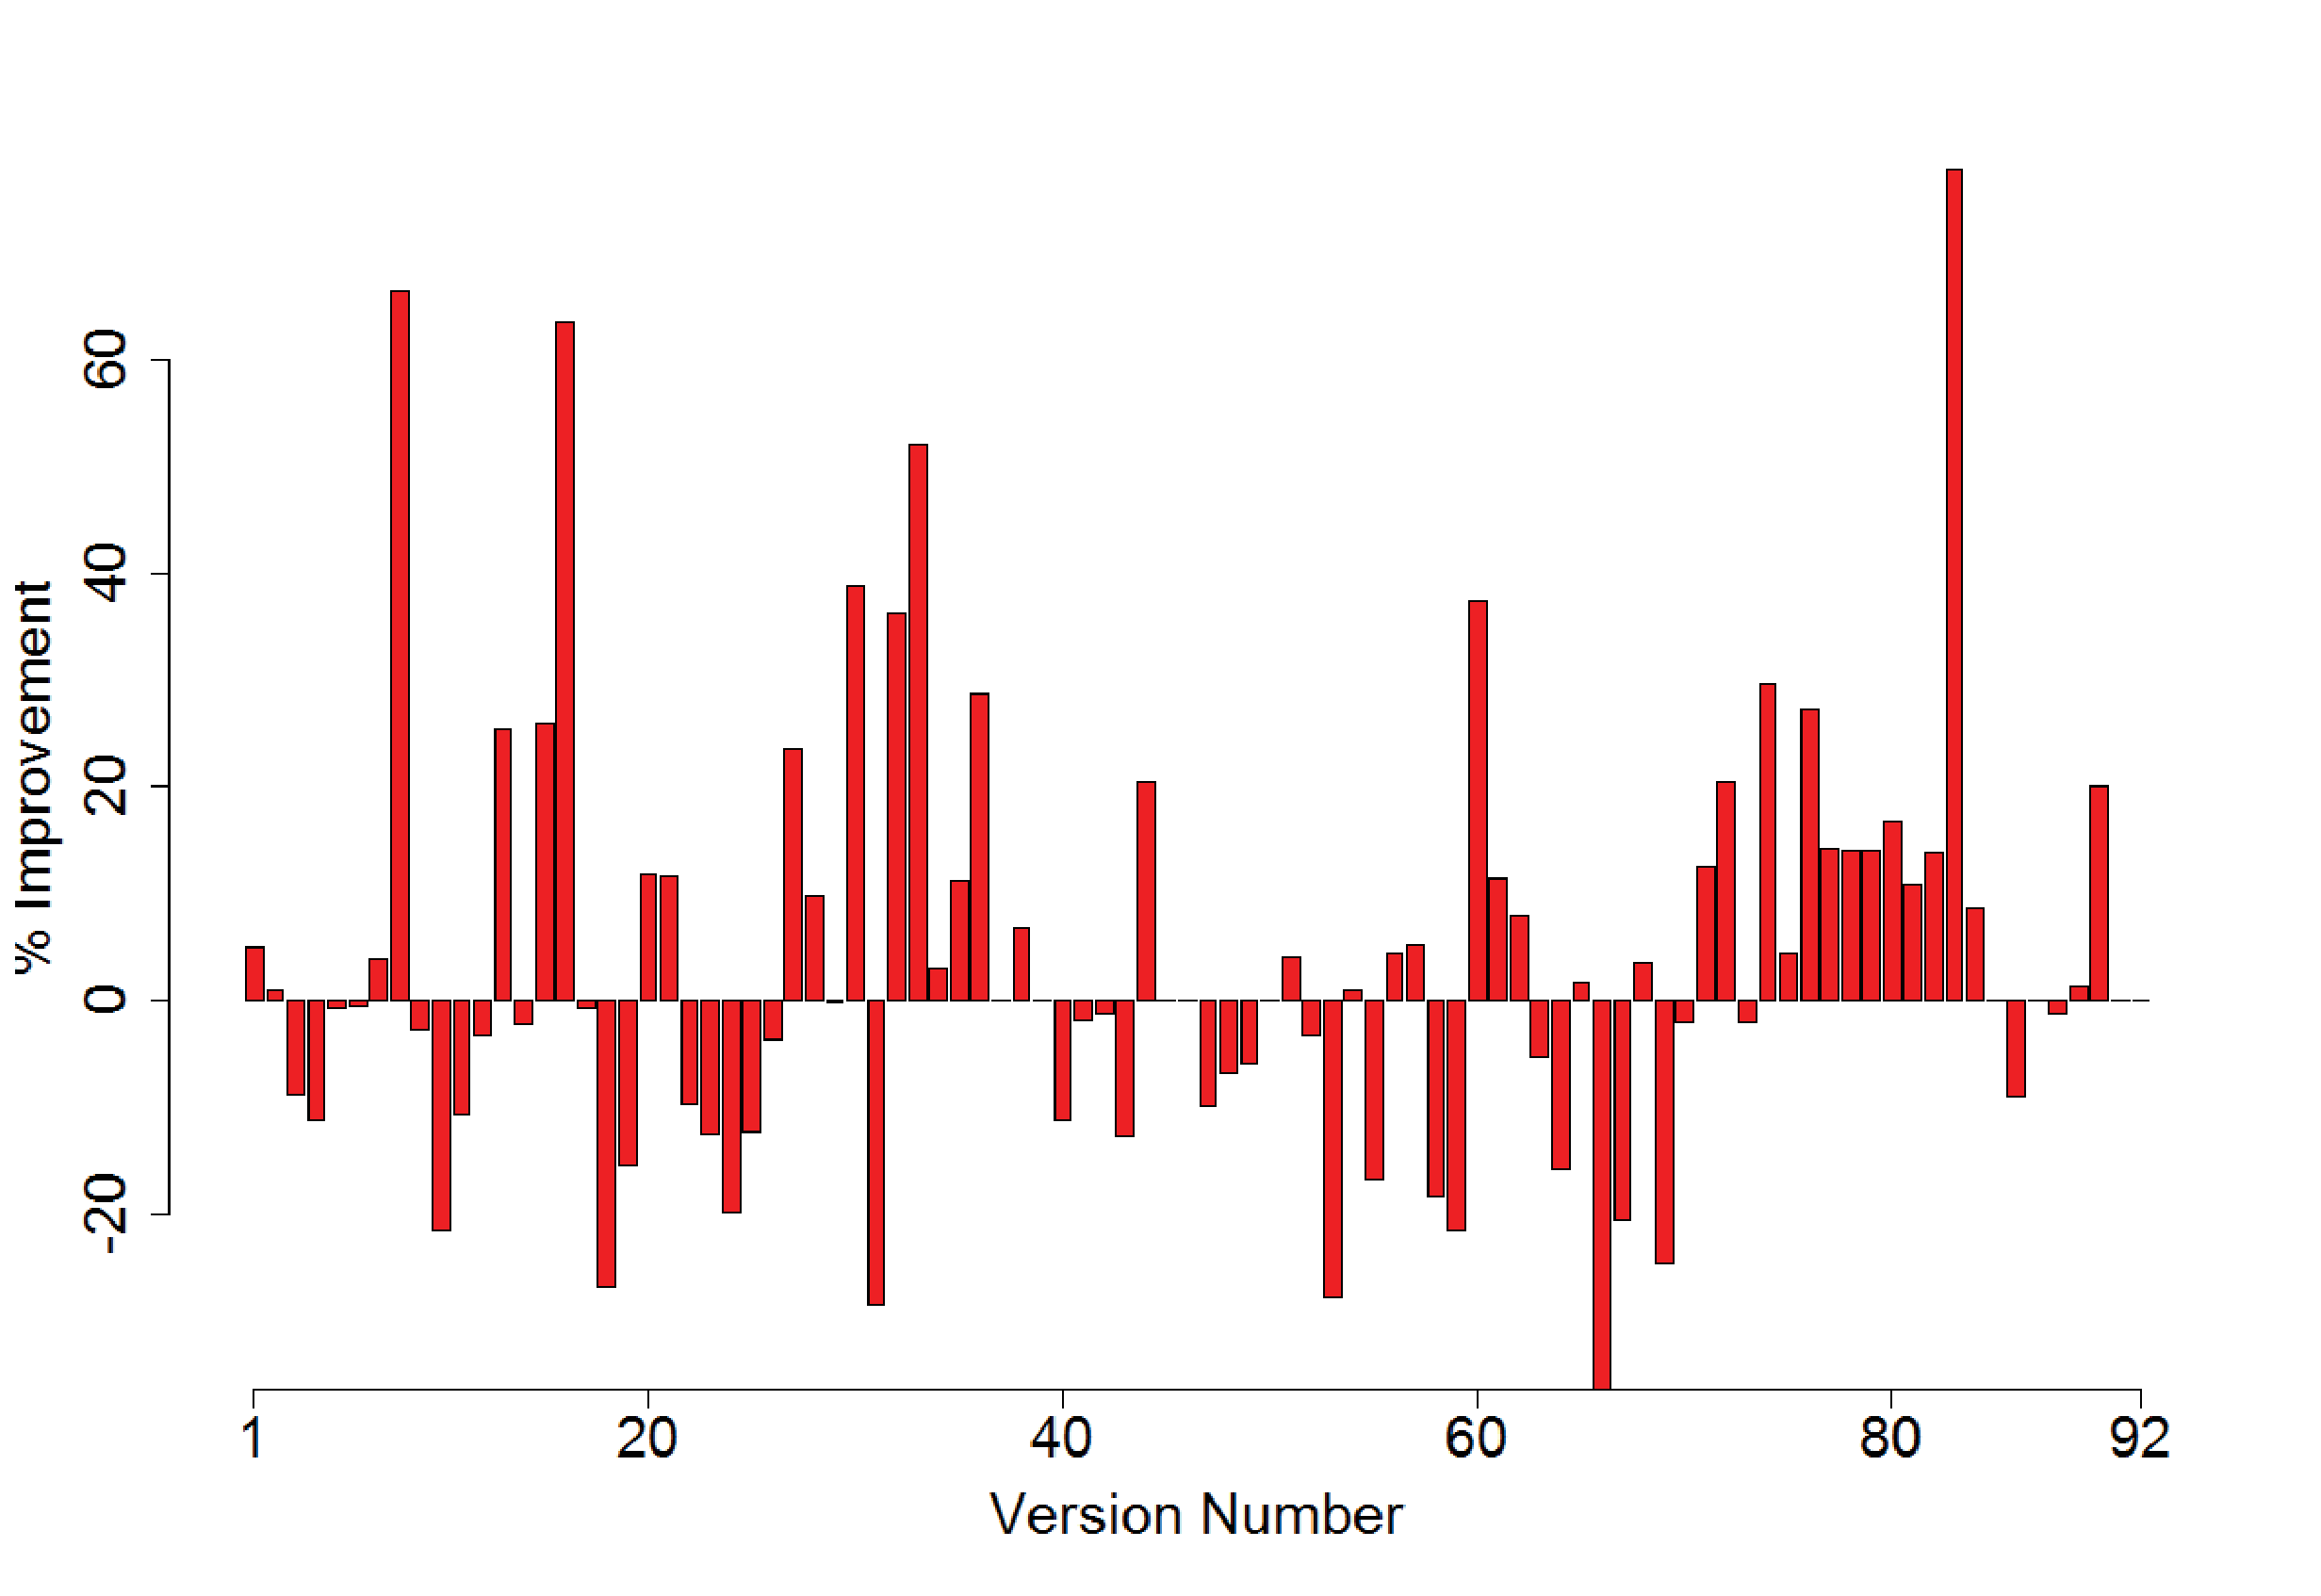
\includegraphics[width=0.6\textwidth]{QRM_allFail.eps}
\caption{Relative performance of NUMFL-GPS-QRM with and without data from passing runs, on individual single-fault program versions.}
\label{QRM_allFail}
\end{figure*}

From Table \ref{table3} and Figure \ref{QRM_allFail}, we can see that NUMFL works fairly well for most subject programs when used with data from only failing runs, although its performance is generally better with data from both passing and failing runs.  Note that with many numerical programs the tolerance for output errors is very small (between 1.0E-5 and 1.0E-12).  For such programs, the output errors from passing runs are clustered around 0, while output errors from failing runs are larger and more varied.  Consequently, the data from failing runs carries more information about the dose-response function than does the data from the passing runs.  Hence, using only data from failing runs to estimate the DRF does not necessarily result in severe bias.

\subsection{Application of NUMFL-GPS to Programs with Multiple Faults}
The empirical results presented in Section \ref{VD} indicate that NUMFL-GPS performs better than the baseline techniques on the subject program versions containing a single fault.  This section reports on the application of NUMFL-GPS to subject program versions with multiple faults.  For this sub-study, we selected five of the larger subject programs (shown in Table \ref{table4}) and generated 5 faulty versions of each for a total of 25 faulty versions.  To create each faulty version, we randomly injected two simulated faults. (Injecting a larger number of faults in our programs tended to make them fail badly on all inputs).  Table \ref{table4} shows the average cost, over the faulty versions of each subject program, of localizing the first fault to be found, for NUMFL-GPS-QRM and each of the baseline techniques.  The table shows that NUMFL-GPS-QRM outperformed the other baseline techniques on average, although SOBER and Ochiai each performed better on one of the subject programs.
\begin{table*}[htbp!]
\fontsize{8pt}{9pt}\selectfont
\centering
\caption{AVERAGE FAULT LOCALIZATION COSTS OF NUMFL-GPS-QRM AND BASELINE METRICS ON SINGLE-FAULT PROGRAM VERSIONS}
\label{table4}
      \begin{tabular}{|l|c|c|c|c|c|c|}
      \hline
\multirow{2}{*}{{\bf Subject Program}}	&	\multicolumn{6}{|c|}{{\bf Technique}}	\\	\cline{2-7}
&{NUMFL-GPS-QRM}	&Ochiai&	Dstar&	ESP(SIV) &	ESP(SCP)	&SOBER \\\hline
Apache\_EigenDecompose	&	10.3\%	&	20\%	&	19.4\%	&	28.3\%	&	25.8\%	&	6.3\%	\\	\hline
Apache\_DScompiler	&	4.5\%	&	31.5\%	&	23.2\%	&	19.9\%	&	10.4\%	&	9\%	\\	\hline
Apache\_Rotation3D	&	7\%	&	3.6\%	&	33.6\%	&	17.5\%	&	17.9\%	&	25.8\%	\\	\hline
Ojaljo\_SchurDecompose	&	5.4\%	&	22.7\%	&	27.1\%	&	8.4\%	&	9.6\%	&	27.1\%	\\	\hline
Jama\_MatrixDecompose	&	14.1\%	&	26.3\%	&	16.5\%	&	26.3\%	&	26.2\%	&	15.5\%	\\	\hline
Average Cost	&	8.3\%	&	20.8\%	&	24\%	&	20.1\%	&	18\%	&	16.7\%	\\	\hline
\end{tabular}
\end{table*}

Figure \ref{QRM_VS_Base_MultipleFault} graphically contrasts the performance of NUMFL-GPS-QRM on the individual two-fault program versions with that of the baseline metrics.  It is evident that SOBER's performance is the second best after NUMFL-GPS-QRM.  Over all 25 faulty subject-program versions, NUMFL-GPS-QRM performed better than SOBER on 15 versions but performed worse on 10 versions.  There were 8 versions for which NUMFL-GPS-QRM performed at least 10\% better than SOBER but only one version for which SOBER performed at least 10\% better than NUMFL-GPS-QRM.  Both Ochiai and ESP-SCP performed better than NUMFL-GPS-QRM on 8 versions but performed worse on 17 versions.  NUMFL-GPS-QRM performed better than ESP-SIV on 19 versions and performed better than DStar on 21 versions.
\begin{figure*}[!thpb]
\centering
\includegraphics[width=\textwidth]{QRM_VS_Base_MultipleFault.eps}
\caption{Performance of GPS-QRM relative to baseline metrics on individual two-fault program versions .}
\label{QRM_VS_Base_MultipleFault}
\end{figure*}

\subsection{Comparison of NUMFL-GPS and NUMFL-CBPS}
In this section, we report the results of empirically comparing the performance of NUMFL-GPS-QRM with that of NUMFL-CBPS-QRM.  We applied the two techniques to the subject program versions with single faults as well as to the versions with two faults.  The average fault localization costs on the single fault versions is shown in Table \ref{table5}.  There were 13 versions for which NUMFL-GPS-QRM performed better than NUMFL-CBPS-QRM. There were only 3 versions for which NUMFL-CBPS-QRM performed better than NUMFL-GPS-QRM. Figure \ref{CBPS_VS_GPS} graphically contrasts the performance of the two methods on the single fault versions.  NUMFL-GPS-QRM performed better on 61 versions, while NUMFL-CBPS-QRM performed better on 31 versions.  NUMFL-GPS-QRM performed at least 20\% better than NUMFL-CBPS-QRM on 15 versions, whereas NUMFL-CBPS-QRM performed at least 20\% better than NUMFL-GPS-QRM on just 4 versions.

\begin{table*}[htbp!]
\caption{AVERAGE FAULT LOCALIZATION COSTS OF NUMFL-GPS-QRM AND NUMFL-CBPS-QRM ON SINGLE-FAULT PROGRAM VERSIONS }
\label{table5}
\centering
      \begin{tabular}{|l|c|c|}
      \hline
\multirow{2}{*}{{\bf Subject Program}}	&	\multicolumn{2}{|c|}{{\bf NUMFL}}	\\	\cline{2-3}
&  GPS-QRM	&CBPS-QRM \\ \hline
Apache\_EigenDecompose	&	12.3\%	&	8.8\%	\\	\hline
Apache\_DScompiler	&	11\%	&	12\%	\\	\hline
Apache\_BigMatrix	&	11.4\%	&	9.9\%	\\	\hline
Apache\_Rotation3D	&	8\%	&	18.9\%	\\	\hline
Ojaljo\_SchurDecompose	&	11.4\%	&	14\%	\\	\hline
Jama\_MatrixDecompose	&	14.2\%	&	23\%	\\	\hline
SciMark\_LU	&	15.3\%	&	27.8\%	\\	\hline
SciMart\_FFT	&	9.5\%	&	19.8\%	\\	\hline
Apache\_SymmLQ	&	2.6\%	&	4.4\%	\\	\hline
Apache\_SplineInterpolator	&	31.7\%	&	35\%	\\	\hline
Apche\_SimpleRegress	&	4.3\%	&	17\%	\\	\hline
Apache\_SchurTransformer	&	3.3\%	&	14.9\%	\\	\hline
Apache\_MillerUpdatRegress	&	7.5\%	&	9.9\%	\\	\hline
Apache\_HarmonicFitter	&	27.3\%	&	32\%	\\	\hline
Apache\_FastSine	&	1.5\%	&	13\%	\\	\hline
Apache\_FastCosine	&	1.3\%	&	1.2\%	\\	\hline
Average Cost	&	10.8\%	&	16.4\%	\\	\hline
\end{tabular}
\end{table*}

Table \ref{table6} shows the average cost, over the faulty versions of each subject program into which two faults were injected, of localizing the first fault to be found, for both NUMFL-GPS-QRM and NUMFL-CBPS-QRM.  NUMFL-GPS-QRM performed better than NUMFL-CBPS-QRM on the two-fault versions of 4 subject programs. NUMFL-GPS-QRM performed worse than NUMFL-CBPS-QRM on the versions of 1 subject program.  Figure \ref{CBPS_VS_GPS_MultipleFault} graphically contrasts the performance of the two methods on the individual two-fault versions.  NUMFL-GPS-QRM performed better than NUMFL-CBPS-QRM on 13 versions and NUMFL-GPS-QRM performed worse on 12 versions.  NUMFL-GPS-QRM performed at least 10\% better than NUMFL-CBPS-QRM on 7 versions, whereas NUMFL-CBPS-QRM performed at least 10\% better than NUMFL-GPS-QRM on just 1 version.

In summary, NUMFL-GPS-QRM performed better than NUMFL-CBPS-QRM on both single-fault and two-fault programs.  The generalized propensity score model $\pmb{\theta}=\pmb{X}'\pmb{\beta}$ achieved better covariate balance than the multinomial logistic regression model used with CBPS.  This may be due to the composition of the data collected from our subject program versions.  The performance of NUMFL-CBPS was poorest with versions that had no more than about 150 failing executions.  However, although NUMFL-CBPS performed worse than NUMFL-GPS in our study, the former's average fault localization cost was still lower than those of the baseline techniques.
\begin{table*}[htbp!]
\caption{AVERAGE FAULT LOCALIZATION COSTS OF NUMFL-GPS-QRM AND NUMFL-CBPS-QRM ON MULTIPLE-FAULT PROGRAM VERSIONS}
\label{table6}
\centering
      \begin{tabular}{|l|c|c|}
      \hline
\multirow{2}{*}{{\bf Subject Program}}	&	\multicolumn{2}{|c|}{{\bf NUMFL}}	\\	\cline{2-3}
&  GPS-QRM	&CBPS-QRM \\ \hline
Apache\_EigenDecompose	&	10.3\%	&	11.1\%	\\	\hline
Apache\_DScompiler	&	4.5\%	&	5.9\%	\\	\hline
Apache\_Rotation3D	&	7.0\%	&	3.0\%	\\	\hline
Ojaljo\_SchurDecompose	&	5.4\%	&	19.8\%	\\	\hline
Jama\_MatrixDecompose	&	14.1\%	&	23.4\%	\\	\hline
{\bf Average Cost} & 8.26\% &12.64\%\\ \hline
\end{tabular}
\end{table*}

\begin{figure*}[!thpb]
\centering
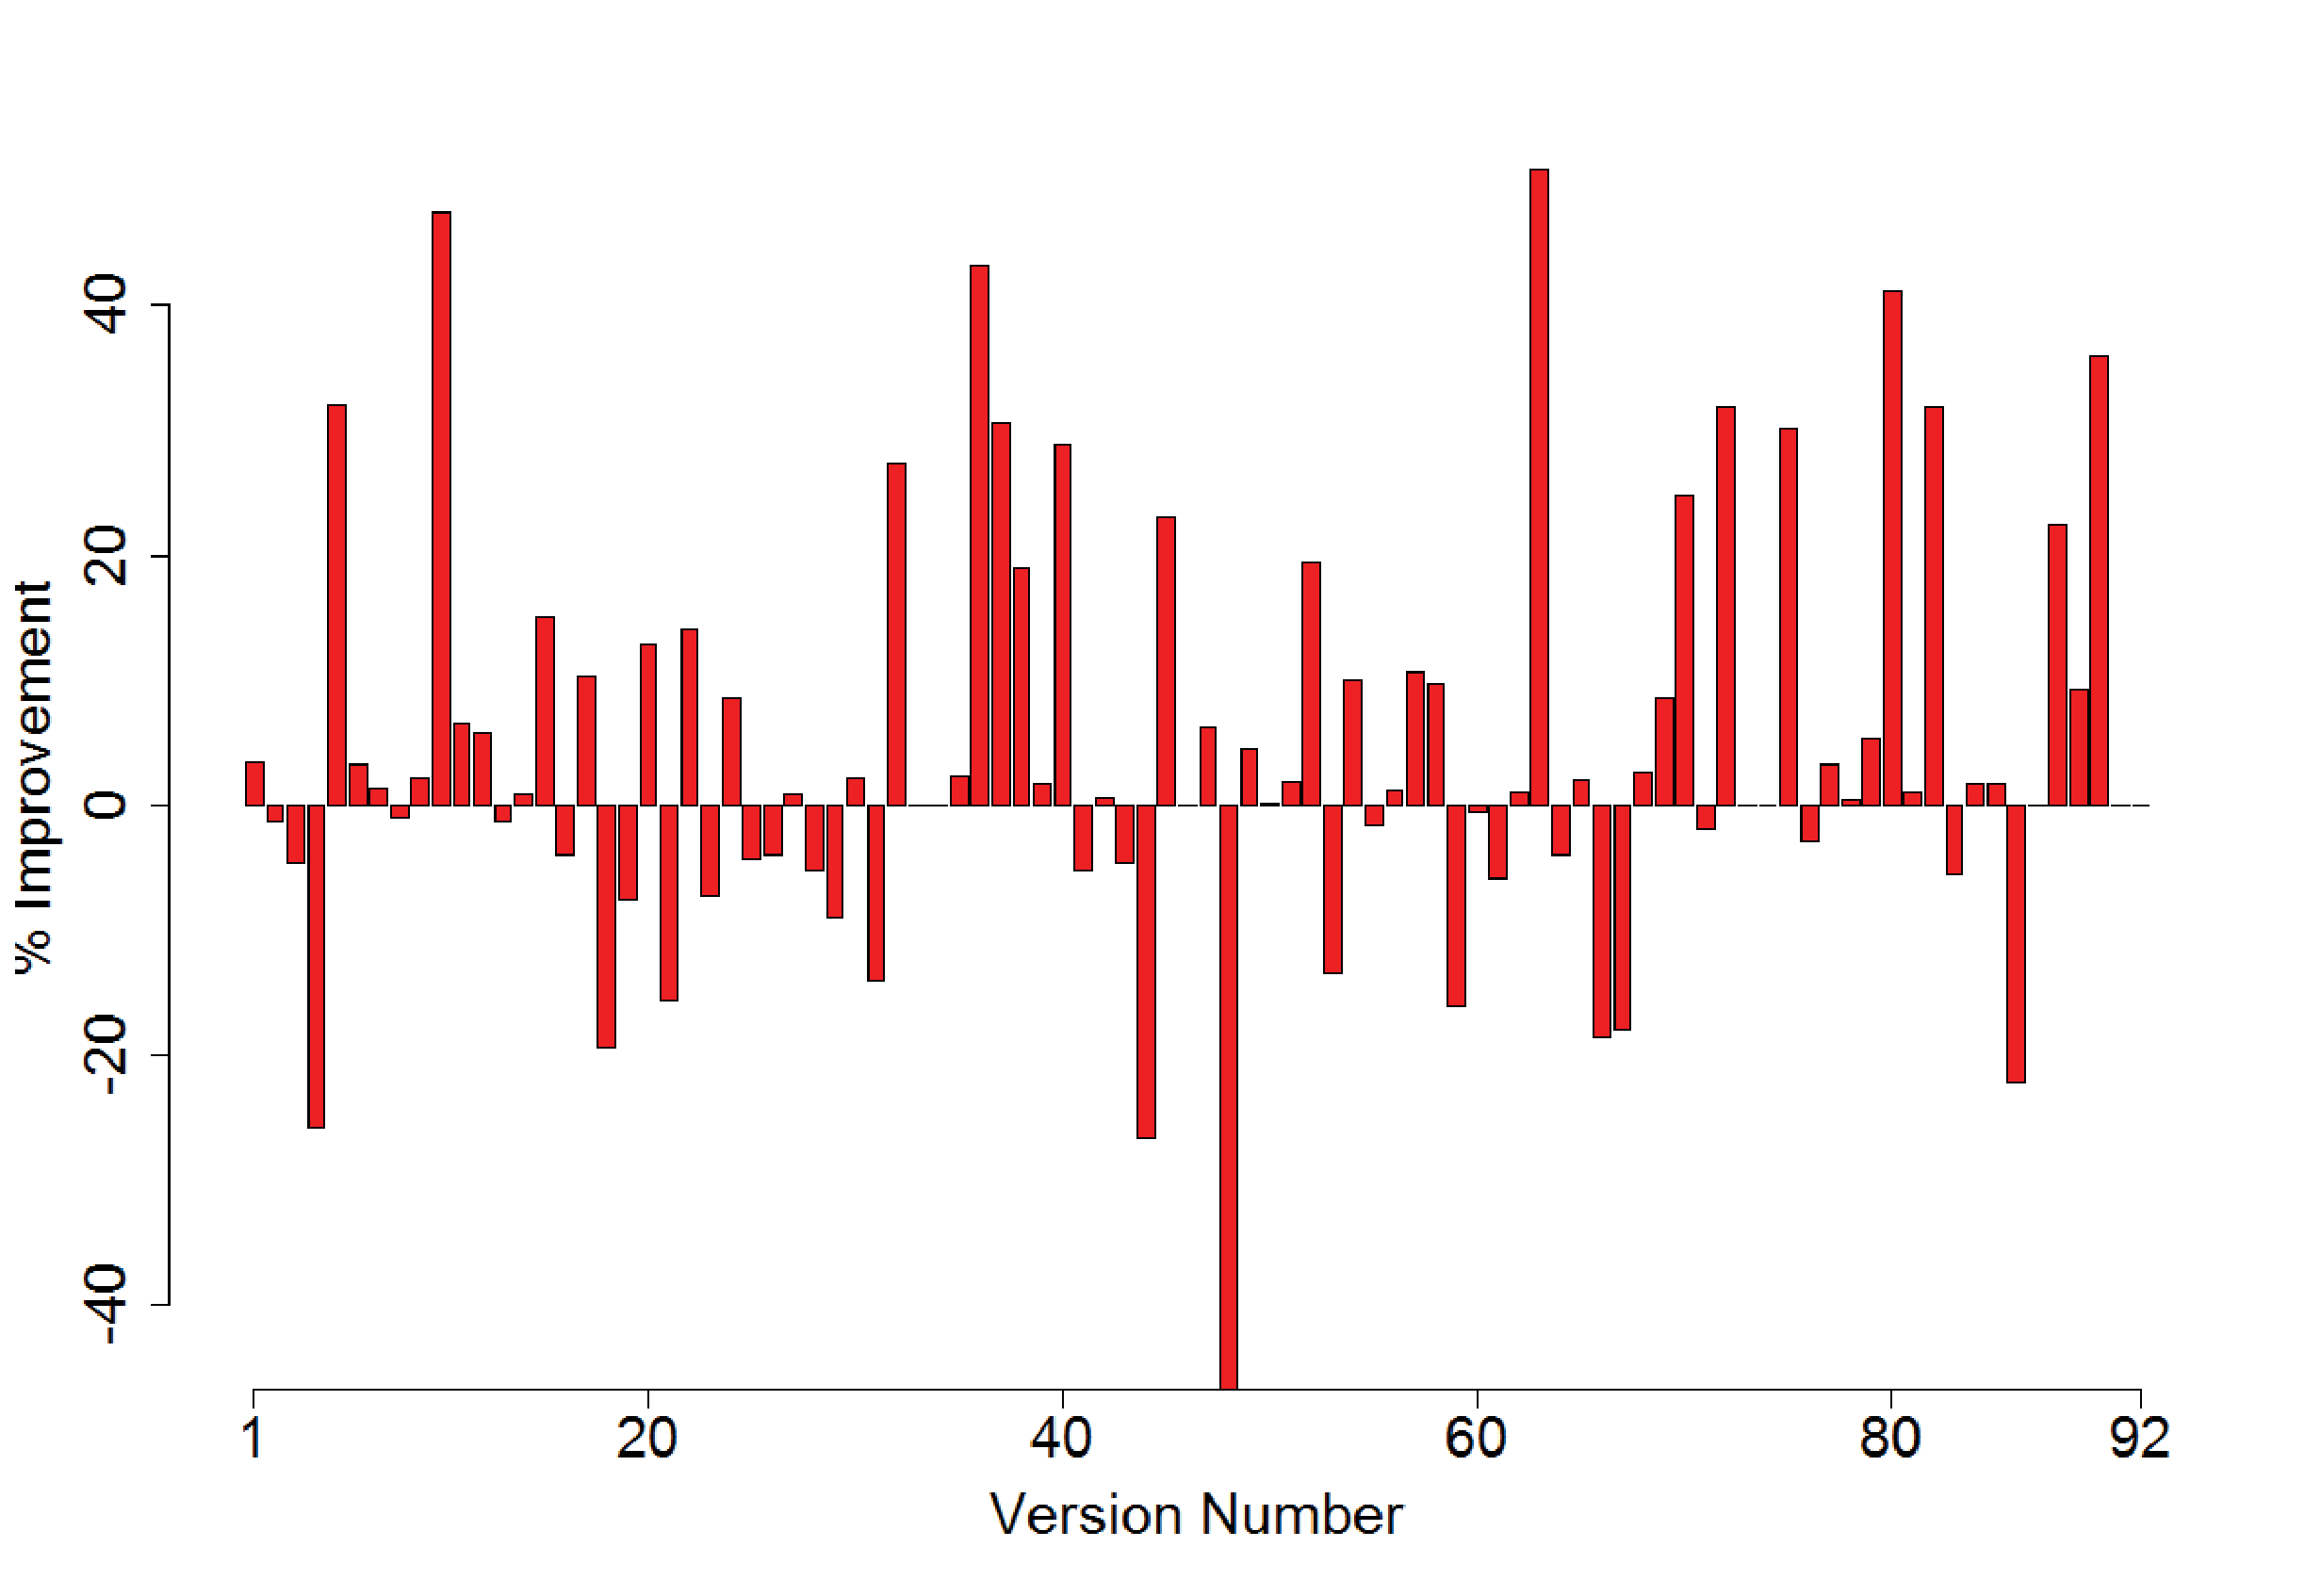
\includegraphics[width=\textwidth]{CBPS_VS_GPS.eps}
\caption{. Relative performance of NUMFL-GPS-QRM and NUMFL-CBPS-QRM on individual single-fault program versions .}
\label{CBPS_VS_GPS}
\end{figure*}

\begin{figure*}[!thpb]
\centering
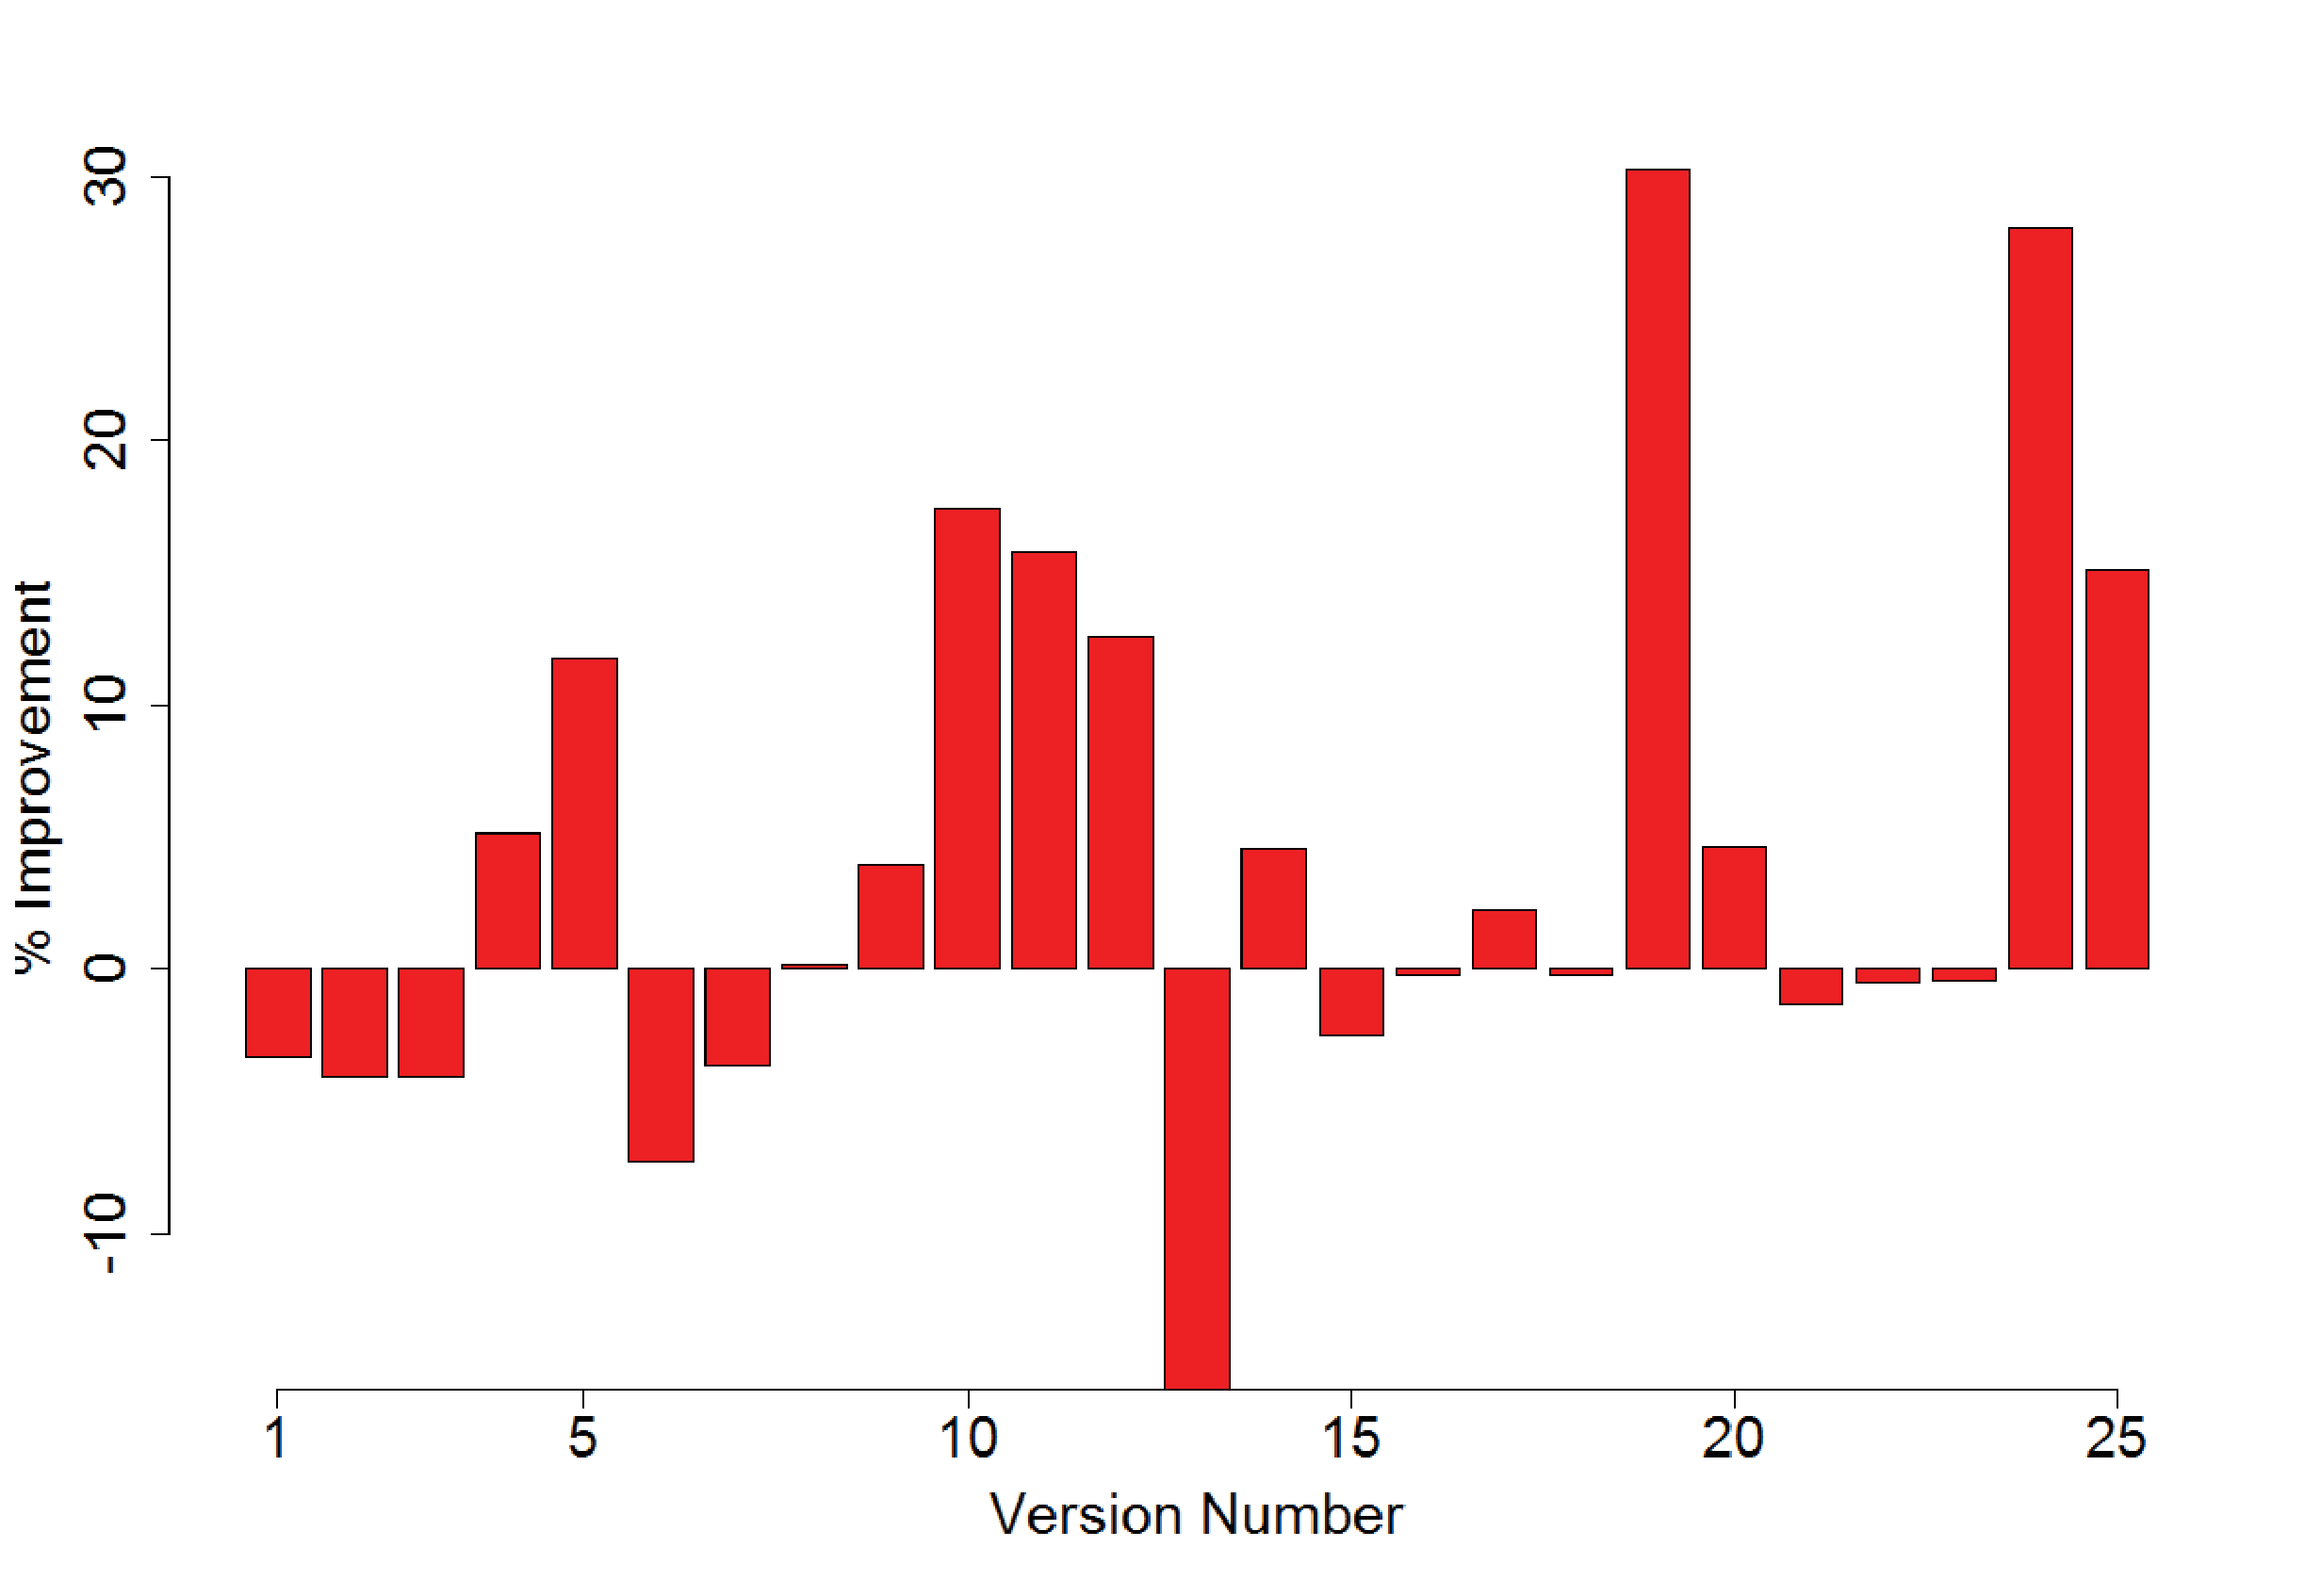
\includegraphics[width=\textwidth]{CBPS_VS_GPS_MultipleFault.eps}
\caption{Relative performance of NUMFL-GPS-QRM and NUMFL-CBPS-QRM on individual two-fault program versions .}
\label{CBPS_VS_GPS_MultipleFault}
\end{figure*}

\subsection{Limitations}
NUMFL and its evaluation are subject to several limitations.  First, NUMFL employs regression models for two purposes: estimating generalized propensity scores and estimating the causal effect of the treatment on the outcome.  We used Gaussian (Normal) linear models for both purposes in NUMFL-GPS, because they are supported by fast and robust software, and they performed well in our empirical study. In NUMFL-CBPS, we use multinomial logistic regression propensity score models.  However, other model choices may be more appropriate for applying NUMFL to different numerical software.  Determining that would require preliminary analysis of the data.  A related issue is that sufficient data must be available to adequately fit each model.  We have found that the number of failing tests should at least 100 to fit adequate regression models.  This is not a serious problem, since faults in numerical programs are usually not guarded by many branch conditions that are likely to cause ``coincidental correctness."  A limitation of our empirical study is that the seeded faults were of three basic types.  In future work, we intend to evaluate NUMFL on subject programs with more varied faults.  Finally, validity of NUMFL (with QRM) depends on Assumptions 1 and 3 in section \ref{twoversion}.  These assumptions do not always hold in practice.  For example, if the effect of a numerical fault does not propagate to the output (coincidental correctness), then Assumption 3 will be violated.

\section{RELATED WORK}\label{relatedwork}
The seminal SFL research of Jones et al. \cite{Jones2002}, which is coverage based, and of Liblit et al. \cite{Liblit2005}, which is predicate based, has inspired much subsequent research.  The use of causal inference methodology in SFL is due to Baah et al. \cite{Baah2010}.  They showed that estimating the AFCE of covering a statement $s$ using a linear regression model that adjusts for coverage of the direct control dependence predecessor of $s$ is effective for reducing confounding bias that often distorts fault localization scores.  Later, Baah et al. \cite{Baah2011} extended this work by using covariate matching to control confounding bias involving both control and data dependence predecessors.  More recently, Gore et al. \cite{Gore2012} extended Baah's initial approach by providing a model that reduces what they called ``failure flow confounding bias," which involves predicate outcomes.  Recently, Shu et al. \cite{Shu2013} proposed a method-level causal inference model to localize faulty methods in large programs. The aforementioned techniques, unlike NUMFL, do not use values of program variables in fault localization.

State-altering techniques, such as {\it cause-transitions} \cite{Cleve2005} and {\it value replacement} \cite{Jeffrey2008} are among the few fault localization techniques based on values of variables.  Cause-transitions employs {\it delta debugging} \cite{Zeller2002} to isolate the cause of a program failure. Value replacement localizes faults by switching program states and re-running the program. Unlike SFL techniques, these techniques actually alter program states, and they require an oracle to determine if alterations cause program failures. On the other hand, they are non-statistical and do not require a sample of both passing and failing executions. The {\it Daikon} system identifies possible invariant conditions in a program based on a sample of executions \cite{Ernst2007}. The {\it DIDUCE} system uses Daikon to report violations of dynamic invariants, which may indicate failures \cite{Hangal2002}. However, these techniques do not address confounding bias.


Some recent studies have developed techniques to analyze instability in floating-point computations. {\it CADNA} \cite{Scott2007} is a library to estimate round-off errors with Monte-Carlo Arithmetic. Tang et al. \cite{Tang2010} proposed a technique to automatically detect such errors by systematically altering the underlying numerical calculation. Lam et al. \cite{Lam2013} proposed to use the detection of significant digit cancellation events to test the precision of numerical programs.  Later, Zhang et al. \cite{Bao2013} extended Lam's work by monitoring the propagation of cancelled bits.  These studies focused on detecting accumulated round-off errors due to finite-precision computation, but they do not address the problem of localizing faults in numerical expressions generally.


Other researchers have proposed alternatives to Imai and van Dyk's approach to defining and using the generalized propensity score.  Hirano and Imbens estimate the causal effect of a continuous treatment variable by fitting one regression model with the GPS as a predictor \cite{Hirano2004}. This method requires discretizing the treatment variable when calculating the propensity score.  Zhao and Imai extend Hirano and Imbens's work by using a smooth coefficient model (SCM) in the regression, so the model can estimate the dose-response function of the treatment variable instead of average causal effect \cite{Zhao2013}.  In preliminary work (with different subject programs), we found that these GPS methods did not perform as well as Imai and Van Dyk's approach, which is used in this paper.


\section{CONCLUSION}\label{conclusion}
In this paper, we have presented and evaluated a value-based causal model, denoted NUMFL, for localizing faults in numerical software. NUMFL employs generalized propensity scores and covariate balancing propensity scores to control confounding bias involving floating-point program variables that carry erroneous values to correct statements.  NUMFL uses a quadratic regression model (QRM) to estimate the average failure-causing effect of a numerical expression.  We reported the results of an empirical comparison of NUMFL to several competing techniques on both single-fault subject programs and multiple-fault subject programs.  NUMFL performed notably better than the other techniques. We also found that NUMFL-GPS works well with data from failing {\it runs alone}.  Finally, we compared the performance two versions of NUMFL, denoted NUMFL-GPS and NUMFL-CBPS, based on the two aforementioned types of propensity scores. We found that the NUMFL-GPS performed better than NUMFL-CBPS for both single-fault programs and two-fault programs.   In the future work, will seek to extend our empirical results to a broader range of subject programs with more varied fault types.  We intend eventually to evaluate NUMFL in a user study, but given the difficulty of conducting an unbiased one, we think it is desirable to refine NUMFL as much as possible beforehand.  Finally, we will also explore the integration of NUMFL with coverage or predicate based causal SFL techniques. 